\chapter{机器学习理论基础}
\label{chap:statistical-learning-framework}

一个垃圾邮件分类器在已经标注的邮件上很少出错，并不意味着它在明天收到的邮件上也会
表现良好。它可能学到了能用于新邮件的分类规律，也可能只是记住了训练邮件。两种做法在训练集上
都能得到很高的准确率，但我们真正关心的是它们对新邮件的判断。

检验一组没有参与训练的邮件，可以帮助评价当前分类器。不过，一次测试仍没有回答学习
算法能否获得统一的成功保证：如果换一批训练邮件，算法还能得到错误率同样低的分类器吗？机器学习理论研究的
一个中心问题，正是有限观测在什么条件下足以支持对未来表现的判断。为此，需要区分训练
数据、算法选出的分类器以及未来邮件的来源，并把“表现好”和“训练成功概率足够高”分别写成可以
分析的条件。

要区分“这次分类器表现良好”和“算法换一批数据仍能成功”，需要先说明算法收到什么、可以选什么、怎样计算错误。本章用垃圾邮件例子逐一建立这些对象，再把成功标准写成PAC保证。随后检查两个障碍：样本没有提供的信息，算法能否补出；假设空间既要足够丰富又不能任意记忆样本，应怎样选择。章末的研究讨论再说明，这些问题怎样扩展到不同算法和数据条件。

\section{学习问题}
\label{sec:learning-problem}
\label{sec:statistical-learning-problem}

比较两个学习方法，不能只看它们都“从样本学出模型”。一条样本是一封邮件还是一段邮件会话，算法预测类别还是选择动作，评价错误率还是行动损失，都会改变学习问题。本节先说明这些选择，让后续各章的风险与样本量结论有共同的解释依据。

\subsection{基本设定}

学习算法首先要知道一条数据记录包含什么。邮件分类中的一条记录由邮件及其标签组成，
回归中的记录可以是输入与数值响应，聚类则可能只有待分组的对象。所有允许记录构成的范围
称为\emph{观测空间}（observation space），记为$Z$。它同时确定损失函数会读取什么，
也提醒我们不能把单条记录、相互依赖的序列和整个环境都不加区分地当作一个样本。

数据本身还没有规定算法应当交付什么。为了评价学习结果，需要先给出一组用于比较的候选
决策，例如全部阈值分类器、受限参数的回归函数或具有固定中心数的聚类方案。这组候选称为
\emph{比较决策空间}（comparison decision space），记为$\mathcal W$；后文所说的最低
风险和超额风险都相对于它计算。算法实际能够返回的结果范围称为\emph{算法输出空间}
（algorithm output space），记为$\mathcal W_{\mathrm{out}}$。若算法只能从候选集合中
选一个结果，两者相同；若算法可以组合多个候选或交付另一种预测器，输出空间就可能更大。

还要规定一个决策在一条观测上会付出多少代价。这个计分规则称为\term{损失函数}（loss function）：损失越小，表示当前评价标准下的结果越好。数据来源与抽样机制说明算法会看到哪些观测、观测之间有什么关系，以及未来表现针对什么总体。算法能否读取标签、环境信息或辅助变量，也会影响它可以做到什么。下面把这些对象写成正式设定。为了讨论训练失败的概率，还要求损失与算法输出可测，
使相应的概率和期望有定义。分类与独立同分布只是后续先讨论的一种情形。

\begin{definition}[学习问题的形式设定]
\label{def:learning-problem-setting}
一个学习问题至少需要规定观测空间$Z$、比较决策空间$\mathcal W$、算法输出空间
$\mathcal W_{\mathrm{out}}$、损失函数、允许的数据来源、抽样机制和算法可见的信息。

在$Z$与$\mathcal W^+=\mathcal W\cup\mathcal W_{\mathrm{out}}$上约定相应的可测结构，
并要求损失
\[
 \ell:\mathcal W^+\times Z\to\mathbb R
\]
联合可测。

抽样机制规定算法所见观测$S$的联合分布。内部随机数$U$定义在另一个概率空间并独立于
$S$；学习算法$A$是从允许输入到$\mathcal W_{\mathrm{out}}$的可测映射，输出
$A(S,U)$。确定性算法省略$U$。
\end{definition}

这些约定区分了算法收到的信息与定理保证的范围。允许的数据来源可以是全部相关分布，
也可以是某个受限分布族；这是我们要覆盖的生成机制，算法不会因此获得完整分布。
抽样机制说明训练观测之间以及训练与评价数据之间的关系，独立随机数$U$则单独表示
算法内部的随机性。算法实际使用的，是允许读取的观测与内部随机数。

为了建立最先使用的基线，以下令允许的数据来源组成分布族$\mathfrak P$。给定
$\mathcal P\in\mathfrak P$，训练样本由$n$个独立同分布观测组成：
\[
 S=(z_1,\ldots,z_n)\sim\mathcal P^n.
\]
二分类、多分类和一般损失章节都从这一训练与评价同分布的关系出发。迁移学习会分别指定
源域与目标域、多个样本量或环境层抽样，并相应改变评价风险和概率来源。各章共享的是
定义~\ref{def:learning-problem-setting}中对象的职责，不是同一个抽样公式。

这个基准中的$n$数的是独立观测。一封邮件、整段会话和一个环境中的数据块，可能具有
不同的独立性条件；把记录拆成更多行，并不一定增加同样多的独立观测。跨域分析还要
说明源域与目标域满足什么关系，不能直接沿用这里的同分布公式。

比较学习结果时，必须同时固定候选决策与损失。最佳风险、近似误差和容量都相对于所选比较空间计算；“误差小”则可能指全部损失小，也可能只指比空间内最佳者多出的损失小。算法还要说明哪些数据可见、可以返回什么结果。若输出始终属于比较空间$\mathcal W$，称为\term{恰当学习}（proper learning）；若允许输出$\mathcal W$之外、但属于$\mathcal W_{\mathrm{out}}$的决策，称为\term{非恰当学习}（improper learning）。二者都与$\mathcal W$中的最低风险比较，区别在于算法可以交付什么。

评价分类器时，对新观测取平均；评价学习算法时，还要考察换一批训练样本或换一组
内部随机数会怎样；跨域分析又可能对环境的抽样取概率。因此，每个保证都必须注明
对什么取平均或概率：平均表现、较高概率下的表现和每个环境都成立的表现，是不同要求。
后续定理还会补充有界性、凸性或覆盖等条件。下面先处理一个共同的技术问题：
当算法在许多候选中选择时，怎样保证相应的上确界和选择结果可测。

\paragraph{可测性与可分性约定}

为了计算“至少一个候选估计失准”的概率，本部分作如下充分约定：对出现在上确界中的一致有界损失函数类$\mathcal F$，每个$f\in\mathcal F$均可测，并存在可数子类$\mathcal F_0$，使每个$f\in\mathcal F$都能由$\mathcal F_0$中的一列函数逐点收敛得到。涉及学习器、压缩、重构或其他数据依赖输出时，还要求相应映射可测。

可数个可测函数的上确界仍可测。上述逼近条件使有限样本上的上确界可以化为可数上确界；由有界收敛，期望风险的相应上确界也可作同样替换。需要经验风险最小化的存在性证明时，可以在固定枚举的可数子类中选择第一个达到给定容差的决策，从而得到可测的近似ERM。若具体问题不能建立这种可数逼近或可测选择，就需要改用外概率表述，或另外给出适用的经验过程条件。无界损失还必须在相应定理中单独检查可积性和所需矩条件。

\subsection{二分类例子}

下面把统一设定特化到二分类：取$Z=X\times Y$、$Y=\{0,1\}$、
$\mathcal W=\mathcal H$，暂令$\mathcal W_{\mathrm{out}}=\mathcal H$，并令
$\ell(h,(x,y))=\ell_{01}(h(x),y)$，即用零一损失评价预测。垃圾邮件例子将这些
对象逐一具体化，并为后面的可实现与不可知PAC比较基准建立直觉。

学习算法根据已经知道类别的邮件，选择一个用来判断新邮件的假设。即使训练数据中的每个
标签都正确，这些数据也可能不足以确定应该采用哪个假设。

例如，假设我们已经为每封邮件计算了一个介于0和1之间的可疑程度分数。分数越高，只表示
邮件越具有被评分程序视为可疑的特征；它不一定等于邮件是垃圾邮件的概率。为了集中讨论
如何从数据选择假设，暂时把评分程序看成固定的，只调整分类时使用的分界值。分类器把
分数达到分界值的邮件判为垃圾邮件，把低于分界值的邮件判为正常邮件。这个分界值称为
\term{阈值}（threshold）。

考虑一份人为构造的训练集，其中只有四封邮件。分数为0.1和0.3的两封邮件已被人工标为
正常邮件，分数为0.7和0.9的两封邮件已被标为垃圾邮件。阈值取0.4时，前两封邮件的分数
低于阈值，后两封高于阈值，四封都能分对。阈值取0.6时，四封邮件的预测结果也完全相同。
训练集在0.3与0.7之间没有提供邮件，所以这两个假设都符合已经观察到的标签。

现在收到一封分数为0.5、尚未标注的新邮件。阈值为0.4的假设会把它判为垃圾邮件，因为
$0.5\geq0.4$；阈值为0.6的假设会把它判为正常邮件，因为$0.5<0.6$。
表~\ref{tab:threshold-email-decisions}列出了这次比较。我们还不知道新邮件的真实类别，
因此不能断定哪个假设正确；能够确定的是，原来的四封训练邮件不足以区分这两个假设。

\begin{table}[htbp]
 \centering
 \begin{tabular}{cccc}
  \toprule
  邮件分数 & 已知类别 & 阈值0.4的预测 & 阈值0.6的预测\\
  \midrule
  0.1 & 正常 & 正常 & 正常\\
  0.3 & 正常 & 正常 & 正常\\
  0.7 & 垃圾 & 垃圾 & 垃圾\\
  0.9 & 垃圾 & 垃圾 & 垃圾\\
  \midrule
  0.5 & 尚未标注 & 垃圾 & 正常\\
  \bottomrule
 \end{tabular}
 \caption{两个阈值假设对同一组邮件的判断。前四行是人为构造的训练数据，最后一行是
 待预测的新邮件。两个假设在训练集上都正确，却对新邮件给出不同类别。}
 \label{tab:threshold-email-decisions}
\end{table}

一封邮件提供给分类器的信息称为\term{输入}，人工给出的真实类别称为\term{标签}。
在这个例子中，输入是邮件分数，记为$x$；标签记为$y$，约定$y=1$表示垃圾邮件，$y=0$
表示正常邮件。输入空间$X$收集所有允许的输入，标签空间$Y$收集所有允许的类别。
这里$X=[0,1]$、$Y=\{0,1\}$；实际模型的输入也可以是多个特征组成的向量，而不只是一项分数。

一条确定的分类规则称为一个\term{假设}（hypothesis）。它规定每个允许输入应该被预测
成哪一类，因此可以写成函数$h:X\to Y$。例如，$h(0.5)=1$表示这个假设会把分数为0.5的
邮件判成垃圾邮件，并不表示这封邮件的真实类别已经被观察到。

\term{假设空间}（hypothesis space）是学习算法允许选择的假设的集合，记为非空集合
$\mathcal H$。如果只允许调整阈值，那么每个阈值对应一个假设，全部阈值假设构成阈值假设空间：
\begin{equation}
 \mathcal H_{\mathrm{thr}}=\{h_t:t\in[0,1]\},\qquad
 h_t(x)=\begin{cases}
  1,&x\geq t,\\
  0,&x<t.
 \end{cases}
 \label{eq:threshold-hypothesis-class}
\end{equation}
下标$t$用来区分不同假设。前面的两个阈值假设分别是$h_{0.4}$和$h_{0.6}$。
学习算法要决定的是选哪个$t$，选定以后才用相应的$h_t$预测新邮件。

只考虑基于阈值的假设，已经加入了一项限制：较高分数的邮件不会在越过阈值后被判为
正常邮件。训练数据本身没有强迫我们采用这个限制。例如，一个只记住四封邮件但对其他邮件
随意分类的假设，也可能在这四封邮件上全部正确。预先限制假设空间或规定假设的选择偏好，称为
\term{归纳偏置}（inductive bias）。它使算法在样本没有直接给出答案的地方，仍能按照
某种确定的原则作出判断。

奥卡姆剃刀常被用来表达优先选择简单解释的思想。在这里，“简单”必须落实到具体假设：
一个阈值只需确定一个分界值，逐条记忆则需要保存每个训练输入。但描述长短依赖采用的编码，
不能脱离表示方式，把“简单”本身当成泛化定理。学习理论还要证明所采用的限制为什么有效。

\paragraph{损失、期望风险与经验风险}

比较假设之前，需要约定怎样计算一次预测的错误。\term{损失}（loss）给每次预测
赋予一个代价。对于当前的二分类任务，我们暂时把两类错误同等对待：把正常邮件错判为垃圾
邮件，或把垃圾邮件错判为正常邮件，都记一次错误；分类正确则不记错误。这种计分方式称为
\term{零一损失}（zero-one loss）。设$h(x)$是预测标签、$y$是真实标签，其公式为
\begin{equation}
 \ell(h,(x,y))=\ell_{01}(h(x),y)=\begin{cases}
  1,&h(x)\neq y,\\
  0,&h(x)=y.
 \end{cases}
 \label{eq:zero-one-loss}
\end{equation}
如果误删正常邮件的代价更高，就应另设损失；以下结论先以零一损失为评价标准。

一封邮件上的损失不能代表分类器的整体表现。假设一个分类器在100封已标注邮件中分错了
3封，那么它在这批数据上的平均损失为$3/100=0.03$。这个数可以直接计算，却只描述已经
检查过的100封邮件。我们还希望知道：从今后会遇到的邮件中随机取出一封，这个分类器
分错它的概率是多少？后一个问题必须考虑不同邮件出现的频率，而不只是当前样本中的计数。

用分布$\mathcal P$表示输入及其真实标签的来源。它描述哪些分数的邮件更常出现，以及
这些邮件分别属于哪一类。例如，即使两个假设只在一个很窄的分数区间内不同，如果大量邮件
都集中在该区间，它们的整体表现仍可能差别很大。分布作用于输入与标签组成的观测
$z=(x,y)\in Z=X\times Y$，通常不为学习算法所知。

对未来邮件的分布取平均，分类器$h$的期望风险就是随机邮件被分错的概率：
\begin{equation}
 R_{\mathcal P}(h)
 =\mathbb E_{(x,y)\sim\mathcal P}[\ell_{01}(h(x),y)]
 =\mathbb P_{(x,y)\sim\mathcal P}(h(x)\neq y).
 \label{eq:population-classification-risk}
\end{equation}

对样本$S=(z_1,\ldots,z_n)$，其中$z_i=(x_i,y_i)$，经验风险相应地写为
\begin{equation}
 \hat R_S(h)=\frac1n\sum_{i=1}^n\ell_{01}(h(x_i),y_i).
 \label{eq:empirical-classification-risk}
\end{equation}
它就是分类器在这份样本上分错的观测数占样本总数的比例。

两个记号的下标说明它们依赖什么：$R_{\mathcal P}$依赖数据分布，$\hat R_S$依赖具体样本。
经验风险中的“经验”表示它由已观察数据计算，而非主观判断。若$S$就是训练集，经验风险
就是训练集上的平均损失；在独立测试集上计算的错误比例则是对未来表现的另一次样本估计，
仍不等于未知的期望风险。

同一个假设的期望风险减去经验风险，称为\term{泛化差}（generalization gap），即
$R_{\mathcal P}(h)-\hat R_S(h)$。这个差值衡量样本上的平均损失与未来平均损失之间的
偏离，可以为正，也可以为负。它不同于后文的超额期望风险：后者比较两个期望风险，
衡量学到的假设距离所选比较基准还有多远。

前面四封邮件上的两个阈值假设，经验风险都是零，但我们还不能算出它们的期望风险。
为了看清缺少什么信息，可以再加入一个明确的教学假设：未来邮件的分数在$[0,1]$上均匀
分布，并且真实类别恰好以0.6为界，分数不低于0.6才是垃圾邮件。此时阈值0.6的假设不会
犯错，阈值0.4的假设则会把分数位于$[0.4,0.6)$的正常邮件误判为垃圾邮件。该区间占
全部概率的$0.2$，所以两个假设的期望风险分别为0和0.2。这个计算依赖刚加入的分布和标签
规律；它不是从那四封训练邮件推导出来的事实。

\paragraph{样本与学习算法}

经验风险要帮助我们判断未来的期望风险，训练邮件就必须与未来邮件存在可说明的联系。最常用的
理想化条件是\term{独立同分布}（independent and identically distributed, i.i.d.）抽样。
“同分布”要求每个训练观测都来自评价未来表现时使用的同一个$\mathcal P$；“独立”要求
这些观测的联合概率按各自概率相乘。用$n$表示训练样本数，这个条件写成
\begin{equation}
 S=\bigl((x_1,y_1),\ldots,(x_n,y_n)\bigr)\sim\mathcal P^n.
 \label{eq:training-sample-distribution}
\end{equation}
它不是对任何数据集都成立的事实。大量重复转发的邮件可能具有依赖，部署后的垃圾邮件
类型也可能变化。后一种变化会使训练与评价不再同分布，需要
第~\ref{chap:transfer-learning-theory}章中的额外分析。

\term{学习算法}（learning algorithm）是根据训练样本选择假设的过程，记为$A$。
算法读取$S$后输出分类器$\hat h=A(S)$。例如，算法可以比较不同阈值在训练邮件上的错误
数，并选出错误数最少的一个；若几个阈值都达到最少错误，它还必须规定如何选择。
算法$A$是选择假设的方法，分类器$\hat h$则是这次训练得到的具体假设，两者不能混为一谈。

本章暂取$\mathcal W_{\mathrm{out}}=\mathcal H$，所以算法进行的是第~\ref{sec:learning-problem}节所说的恰当学习。若假设空间只包含单阈值假设，而算法组合多个假设得到一个不再是单阈值的分类器，就需要扩大输出空间；后文采用这种非恰当输出时会另行说明。

同一个算法用不同训练集可能选出不同分类器。仍以阈值分类器为例，一批邮件可能包含许多接近
真实分界的样本，另一批可能恰好缺少这些邮件；即使算法完全相同，两次训练也可能得到
不同阈值。因此，评价一个已经训练好的分类器，与评价一种学习算法的成功保证，是两个问题。

图~\ref{fig:learning-two-randomness}区分了这两种评价。固定训练结果$\hat h$以后，
期望风险$R_{\mathcal P}(\hat h)$只对一封新的随机邮件取平均。若重新抽取训练集并重新
训练，输出$A(S)$随之改变，期望风险$R_{\mathcal P}(A(S))$也会改变。
学习算法的成功保证取决于第二种变化：随机抽到一份训练集后，它有多大概率产生低期望风险分类器？
算法若还使用内部随机数，这个概率也要包含算法本身的随机性。

\begin{figure}[htbp]
 \centering
 % 两层随机性分别作用于训练输出和固定输出上的新观测。
\begin{tikzpicture}[figure picture,foundation picture]
 \path[use as bounding box] (0,7) rectangle (112,72);
 \node[foundation input,fill=FigureBlueFill,minimum width=30mm] (p) at (54,65) {未知分布$\mathcal P$};
 \node[foundation input,fill=FigureBlueFill,minimum width=28mm] (s) at (20,42) {训练集$S\sim\mathcal P^n$};
 \node[foundation input,fill=FigureBlueFill,minimum width=28mm] (z) at (88,42) {新观测$z\sim\mathcal P$};
 \node[foundation model,minimum width=28mm] (a) at (20,20) {学习算法$A$};
 \node[foundation output,fill=FigureYellowFill,minimum width=30mm] (h) at (54,20) {$\hat h=A(S)$};
 \node[foundation loss,fill=FigureRedFill,minimum width=30mm] (l) at (88,20) {$\ell(\hat h,z)$};
 \draw[foundation flow] (p)--(s); \draw[foundation flow] (p)--(z);
 \draw[foundation flow] (s)--(a); \draw[foundation flow] (a)--(h);
 \draw[foundation flow] (z)--(l);
 \draw[foundation flow] (h.east)--(l.west);
 \draw[foundation frame,dashed] (3,11) rectangle (71,51);
\end{tikzpicture}%

 \caption{评价分类器与评价学习算法所涉及的两层随机性。固定一次训练的结果后，期望风险
 对右侧的新观测取平均；重新抽取左侧训练集则可能得到另一个分类器。学习保证还要控制
 后一种随机性导致训练失败的概率。}
 \label{fig:learning-two-randomness}
\end{figure}

\subsection{一般学习的风险与可学习性}

式~\eqref{eq:population-classification-risk}和\eqref{eq:empirical-classification-risk}
已经在二分类例子中给出了期望风险与经验风险。把分类器$h$换成一般决策$w$，把输入标签对
换成一般观测$z$，就能为分类器、回归函数、聚类中心及其他决策提供统一记号；风险的具体
含义仍由观测和损失决定。

\begin{definition}[一般学习问题的期望风险]
\label{def:general-population-risk}
设$\mathcal P\in\mathfrak P$。对任意$w\in\mathcal W^+$，若$\ell(w,\cdot)$在$\mathcal P$下可积，则$w$的期望风险为
\[
 R_{\mathcal P}(w)=\mathbb E_{z\sim\mathcal P}\ell(w,z).
\]
\end{definition}

\begin{definition}[一般学习问题的经验风险]
\label{def:general-empirical-risk}
给定样本$S=(z_1,\ldots,z_n)\in Z^n$，任意$w\in\mathcal W\cup\mathcal W_{\mathrm{out}}$的经验风险为
\begin{equation}
 \hat R_S(w)=\frac1n\sum_{i=1}^n\ell(w,z_i).
 \label{eq:general-risk}
\end{equation}
\end{definition}

二分类中，标签噪声可能让所有分类器都犯错；一般损失下，也未必存在零风险决策。因此，下面的一般定义不要求算法达到零风险，而是要求它接近比较空间$\mathcal W$中的最低期望风险。同时，成功概率应对允许分布族中的每一个分布都达到要求。

调用下面的定义时，默认$\inf_{w\in\mathcal W}R_{\mathcal P}(w)$有限，随机输出的
期望风险几乎处处有限，且$R_{\mathcal P}(A(S,U))$作为$(S,U)$的函数可测。
具体无界损失还须在相应定理中给出保证这些条件成立的可积性或矩条件。PAC先回答
统计上是否能学到，再检查训练与预测能否由程序实现。

\begin{definition}[相对于分布族的PAC可学习性]
\label{def:general-pac-learnability}
若存在算法$A$，对任意$\varepsilon,\delta\in(0,1)$存在整数$n_0(\varepsilon,\delta)$，使任意$\mathcal P\in\mathfrak P$和$n\geq n_0(\varepsilon,\delta)$均满足
\[
 \mathbb P_{S\sim\mathcal P^n,U}\!\left\{
 R_{\mathcal P}(A(S,U))\leq
 \inf_{w\in\mathcal W}R_{\mathcal P}(w)+\varepsilon
 \right\}\geq1-\delta,
\]
则称该学习问题相对于$\mathfrak P$是PAC可学习的。概率包含训练样本和算法内部随机数；确定性算法省略$U$。只有当$\mathfrak P$包含所讨论空间上的全部相关分布时，才称这一保证为分布无关。
\end{definition}

定义~\ref{def:general-pac-learnability}只规定统计保证。若进一步要求学习程序在给定
编码下停机，且输出的预测程序对每个允许输入都停机，就进入\term{可计算学习}
（computable learning）；若还要求样本量、训练时间和预测时间具有规定参数的
多项式上界，就进入\term{高效学习}（efficient learning）。这三层要求不能相互代替，
第~\ref{sec:pac-computation-requirements}节将用二分类问题给出具体定义。

\section{PAC学习}
\label{sec:pac-learning}

前面的邮件例子留下两层不确定性：一次训练得到的分类器可能仍会误判，换一批训练邮件又可能学出更差的分类器。\term{PAC学习}（probably approximately correct learning）分别限制这两件事：用误差容限$\varepsilon$限制分类器的误差，用失败概率容限$\delta$限制训练失败的概率。在可实现情形中，$\varepsilon$限制全部错误概率；在不可知情形中，它限制相对于假设空间内最佳分类器多出的错误概率。算法应以较高概率达到相应的误差要求。

例如，要求“至少以99\%的概率，得到未来错误率不超过5\%的分类器”，就对应
$\delta=0.01$和$\varepsilon=0.05$。其中5\%评价一次训练得到的分类器，99\%评价
抽取训练集并训练这一整个过程。这个说法既不要求训练样本全部分对，也不保证每一批未来
邮件的实际错误比例都恰好小于5\%。它约束的是分类器在数据分布上的错误概率。

有限样本可能遗漏某些输入，这使无条件、零失败的承诺通常无法满足。PAC允许少量失败，
但要求我们能通过足够多的样本，把失败概率控制到事先指定的水平。至于“误差小”应以零为
目标，还是以当前假设空间能达到的最好结果为目标，则取决于数据是否允许完美分类。
定义~\ref{def:general-pac-learnability}已经给出这两类问题共用的概率量词。特化到二分类时，
比较空间取$\mathcal H$，损失取零一损失；可实现与不可知设定的差别落在允许分布族及其比较基准上。

\subsection{可实现情形}

可实现设定假定假设空间中存在一个不会在数据分布上犯错的假设。在这个条件下，低错误率分类器确实存在；需要解决的是怎样用有限观测选出它或足够好的
近似。标签噪声或假设空间遗漏真实规律造成的误差，暂时由这一假设排除。

\begin{definition}[可实现性]
\label{def:realizability}
如果某个假设能够以概率1正确预测数据来源中的标签，就称数据分布对该假设空间
是\term{可实现的}（realizable）。形式上，分布$\mathcal P$对$\mathcal H$可实现，
是指存在$h^\star\in\mathcal H$满足
\[
 R_{\mathcal P}(h^\star)=0.
\]
\end{definition}

在前面的教学分布中，真实类别以分数0.6为界，而假设空间包含阈值0.6对应的假设，所以该分布对阈值假设空间
可实现。若同一分数下既可能出现正常邮件，也可能出现垃圾邮件，单凭这个分数就无法总是
判断正确；此时可实现性可能不成立。这里要求在总体分布下犯错的概率为零，而不是只要求在某一张训练表上全部分对。
训练集碰巧没有矛盾，并不能证明总体上存在零错误分类器。

即使我们知道零期望风险假设存在，也不知道它是哪一个。学习保证需要说明：无论这个未知分布
具体如何，只要它满足可实现性，一种预先确定的算法就能从足够多的样本中找到低期望风险假设。
“足够多”可以随误差容限$\varepsilon$和失败概率容限$\delta$变化，但不能依赖算法事先
不知道的具体分布。

将定义~\ref{def:general-pac-learnability}中的$\mathfrak P$取为所有对$\mathcal H$可实现的
分布，并把样本量阈值$n_0$记为$m_{\mathcal H}$。由于每个允许分布都满足
$\inf_{h\in\mathcal H}R_{\mathcal P}(h)=0$，公共保证特化为
\begin{equation}
 \mathbb P_{S\sim\mathcal P^n}
 \left(R_{\mathcal P}(A(S))\leq\varepsilon\right)\geq1-\delta.
 \label{eq:pac-guarantee}
\end{equation}
满足这一特化保证时，就说$\mathcal H$在可实现设定下是PAC可学习的。同一个算法必须
适用于所有允许的分布，$m_{\mathcal H}(\varepsilon,\delta)$只依赖误差容限、失败概率容限
及假设空间。

在所有学习算法中，使上述保证对任意更大样本量都成立的最小样本量阈值，称为
\term{样本复杂度}（sample complexity）。证明某个$m_{\mathcal H}(\varepsilon,\delta)$
满足上述条件，就给出了样本复杂度的上界；它未必是所需的最小值。若算法随机化，概率还包含其内部随机性。

式~\eqref{eq:pac-guarantee}应当从内向外读。$A(S)$是本次训练得到的分类器；
$R_{\mathcal P}(A(S))\leq\varepsilon$表示这次训练成功，成功的标准是所得分类器的
期望风险不超过误差容限；在零一损失下，这就是分类错误概率不超过$\varepsilon$。最外层的概率再询问，这个成功事件在随机抽取训练集时有多大概率
发生，并要求它至少为$1-\delta$。

公共定义还规定了算法、样本量与分布之间的先后关系。我们不能先知道真实分布，再为它挑选
专用算法，然后称这个假设空间可学习。同样，样本量上界也不能为每个未知分布临时另定。
分布无关的保证要求同一上界覆盖所有允许分布，这比证明算法在某一个熟悉的数据来源上
有效更强。PAC的计算形式化由Valiant提出；这里采用统计学习教材中常用的分布无关表述
\scite{valiant1984}。

减小$\varepsilon$和减小$\delta$对应不同的改进。前者要求成功时得到更准确的分类器，
后者要求更少发生训练失败。它们对样本量的影响不必相同；具体关系需要从假设空间和学习
算法推导，不能只根据PAC的名称确定。第~\ref{chap:binary-learnability}章将给出有限假设空间
中的样本量计算。

上述PAC保证允许要求任意小的$\varepsilon$，因此属于\term{强学习}（strong learning）。
\term{弱学习}（weak learning）则把任意精度要求放宽为一个固定优势。在二分类的可实现
设定中，若存在$\gamma\in(0,1/2)$、同一个算法$A$和有限样本量函数
$m_{\mathcal H}^{\mathrm{weak}}(\delta)$，使得对任意$\delta\in(0,1)$、任意对
$\mathcal H$可实现的分布$\mathcal P$以及任意
$n\geq m_{\mathcal H}^{\mathrm{weak}}(\delta)$，都有
\[
 \mathbb P_{S\sim\mathcal P^n,A}\!\left(
 R_{\mathcal P}(A(S))\leq\frac12-\gamma
 \right)\geq1-\delta,
\]
就称$\mathcal H$是弱PAC可学习的。这里$\gamma$不能随分布、样本或$\delta$改变；
算法随机化时，概率也包含其内部随机性。例如$\gamma=0.1$时，成功训练的错误率上限
为40\%，优于不看输入、等概率猜两个标签的50\%错误率。第~\ref{sec:boosting}节反复
调用弱学习器时，还会把目标假设空间与算法的输出空间分开写明。每轮改变的是样本权重
所定义的分布；同一个算法和同一个优势必须对这些仍由目标空间实现的分布成立，各轮失败
概率也要纳入总预算，不能把某一次训练略优于随机猜测当作弱学习保证。

\subsection{不可知情形}

可实现PAC保证有一个前提：假设空间中必须存在零期望风险假设。实际应用中，这个前提常常无法确认，甚至已经明确不成立。此时，不能把算法未达到零期望风险简单归因于训练失败；需要先判断当前输入信息与假设空间是否允许零期望风险假设存在。

零期望风险可能因两种原因无法达到：输入表示丢失了区分类别所需的信息，或者假设空间
没有包含所需的决策规律。前者即使知道完整分布也会留下不可消除的错误，后者则使当前
假设空间内的最优风险大于所有可测分类器能够达到的风险。第~\ref{sec:statistical-model-selection}节
会用两个具体例子把这两种来源分别写成贝叶斯风险与近似误差。标注噪声也必须按评价目标
解释：若把带噪声的观测标签作为$y$，噪声已经包含在分布$\mathcal P$中；若训练和评价
使用不同版本的标签，则需要另外说明二者关系，不能直接沿用同分布保证。

这两种困难要求学习保证改变比较基准。我们仍然希望算法善用数据，但不再承诺假设空间中存在零期望风险假设，也不预先规定噪声应符合哪一种模型。\term{不可知设定}（agnostic setting）就是在这样的条件下，要求学习结果接近当前假设空间能够达到的最低期望风险。“不可知”所放弃的是关于零期望风险目标假设的先验承诺，不是训练标签，也不是独立同分布假设。

假设当前假设空间能达到的最低期望风险为8\%。若仍要求分类器的期望风险不超过2\%，这个
目标就无法实现。更合理的要求是：算法的期望风险比假设空间内最低值至多高2个百分点，也就是不超过
10\%。学习结果高于假设空间内最低期望风险的差值，称为相对于假设空间的\term{超额期望风险}
（excess risk）；这里允许的超额期望风险上限是2个百分点。这个差值度量学习结果还落后于
同一假设空间中的最佳结果多少。

假设空间内最低期望风险记为$R_{\mathcal P,\mathcal H}^\star$。某些无限假设空间中的期望风险可以
不断接近一个值，却没有成员恰好达到它，因此用下确界而不是最小值定义这个比较基准：
\begin{equation}
 R_{\mathcal P,\mathcal H}^\star=\inf_{h\in\mathcal H}R_{\mathcal P}(h).
 \label{eq:best-in-class-risk}
\end{equation}
例如一列假设的期望风险为$0.08+0.1/k$并随$k$增大接近0.08，0.08就可以是下确界，即使没有
假设的期望风险恰好等于0.08。这个数学例子说明，下确界允许我们讨论最佳可逼近水平，而不额外
假定最优假设一定存在。

若将定义~\ref{def:general-pac-learnability}中的$\mathfrak P$取为$X\times Y$上的全部
相关联合分布，并把样本量阈值记为$m_{\mathcal H}^{\mathrm{agn}}$，公共保证相应地写成
\begin{equation}
 \mathbb P_{S\sim\mathcal P^n}\left(
 R_{\mathcal P}(A(S))\leq R_{\mathcal P,\mathcal H}^\star+\varepsilon
 \right)\geq1-\delta.
 \label{eq:agnostic-pac-guarantee}
\end{equation}
满足这一特化保证时，就说$\mathcal H$是\term{不可知PAC可学习的}
（agnostic PAC learnable）。这里的误差容限$\varepsilon$约束超额期望风险，而不是
分类器的全部期望风险。

这个保证也覆盖可实现分布。此时假设空间内最低期望风险为零，式~\eqref{eq:agnostic-pac-guarantee}就恢复为可实现PAC保证。因此，不可知学习扩大了需要覆盖的数据分布范围，对算法的统一能力提出了更强要求；它并不是把成功标准任意降低。算法不需要事先知道假设空间内最低期望风险的数值，正如可实现学习不需要事先知道哪个假设具有零期望风险；这个数值用于评价算法的结果。

\subsection{计算要求}
\label{sec:pac-computation-requirements}

前面的统计保证主要回答有限数据是否足以支持可靠预测。在这种表述中，学习算法只是
从样本到分类器的一个映射；证明这样的映射存在，还没有提供计算机能够执行的程序。

把映射落实为程序，还要回答程序是否停机，以及所需计算量怎样随问题规模增长。
可计算PAC学习与高效PAC学习分别补充这两层要求，同时保留相应的PAC期望风险保证。

讨论程序之前，必须说明数据和假设怎样编码。以自然数输入为例，每个输入可以写成二进制字符串，标签只需一个比特；一个分类器则可用计算其预测的程序表示。学习程序的输出是这个预测程序的有限描述。任意实数不一定有有限的精确编码，因此不能把连续输入中的一次任意精度计算默认当作常数时间操作；必须另行约定精度或计算模型。

\begin{definition}[可计算PAC学习]
\label{def:computable-pac-learning}
在固定的有效表示下，如果存在一个可执行的学习程序，能够在每个允许的有限训练样本上停机，输出一个对每个允许输入都能停机并给出标签的预测程序，并且该学习算法满足PAC保证，就称该假设空间是可计算PAC可学习的（computably PAC learnable），简称CPAC可学习。这里的PAC保证可以采用可实现版本或不可知版本，使用时必须说明采用哪一种。
\end{definition}

这个定义同时约束训练和预测。仅仅说“输出期望风险最小的假设”没有告诉计算机怎样找到该假设；仅仅输出一段可能永远不返回预测的代码，也没有给出可用的分类器。另一方面，可计算性允许非常缓慢但最终会完成的计算，并不要求多项式时间。若还要求输出属于$\mathcal H$，得到恰当CPAC学习；允许输出假设空间之外的分类器时则得到非恰当版本。本章仍沿用恰当输出的默认约定，比较文献结论时需要检查这一约定。

学习程序能够执行，与所需样本量上界能够计算，也有区别。前者保证拿到一份样本后能够完成训练，后者使我们能根据$\varepsilon,\delta$计算一个足够大的样本数。基本CPAC定义不自动要求后者；文献还研究附加可计算样本上界的版本。这些区分及其分离结果可见Delle Rose等的研究\scite{dellerose2023}。第~\ref{sec:computable-binary-learning}节将用可计算的缺失标记继续分析它们。

即使训练程序一定停机，穷举搜索仍可能过慢。假设一个假设空间由$d$比特索引指定，共有$2^d$个假设，并且给定索引后可以在多项式时间内计算预测。逐一计算全部假设的经验风险就能完成有限搜索，但需要检查指数多个假设。定理~\ref{thm:finite-realizable-pac}将说明，在可实现情形下，充分样本量只按
\[
 \frac{d\log2+\log(1/\delta)}{\varepsilon}
\]
增长。样本数对$d$的线性依赖与穷举计算量的指数依赖并不矛盾：观察多少数据和怎样搜索假设是两种资源问题。这只说明穷举算法很慢，不能由此断言该假设空间不存在更快的学习算法。

\begin{definition}[高效PAC学习]
\label{def:efficient-pac-learning}
高效PAC学习（efficient PAC learning）要求在满足PAC期望风险保证的同时，样本量、训练计算量及输出分类器的预测计算量都有多项式上界。为明确规模依赖，考虑由参数$d$描述的一族假设空间$\mathcal H_d$，并约定观测编码长度上界为$b$。本书采用的高效性约定要求存在统一程序和固定多项式$p,q$，使所需样本量及训练时间分别满足
\begin{equation}
 \begin{aligned}
 m_{\mathcal H_d}(\varepsilon,\delta)
 &\leq p\bigl(d,b,1/\varepsilon,\log(1/\delta)\bigr),\\
 T_{\mathrm{train}}
 &\leq q\bigl(n,d,b,1/\varepsilon,\log(1/\delta)\bigr).
 \end{aligned}
 \label{eq:efficient-pac-resources}
\end{equation}
学习程序把$d,\varepsilon,\delta$及样本编码作为输入；若程序不显式接收$\varepsilon,\delta$，而由外部按精度与失败概率要求选择
样本量，也须说明样本量怎样根据这两项要求确定。输出分类器属于预先规定、可统一求值的表示族，它在新输入
上的求值时间应被$d$、输出表示长度和输入编码长度的某个固定多项式所控制，不能仅把任意
程序的短代码长度当作预测高效的依据。若这族假设空间还由目标描述长度等量参数化，也须将
它们明确列入规模变量。
\end{definition}

这里的$d$表示已经约定的假设空间规模参数，不总是特征维数；$b$避免把任意长度的数值读写与比较算作一次免费操作。多项式的次数不能随着$d$增大而增大，否则“对每个固定$d$都能运行”仍可能掩盖指数增长。不同文献对失败概率参数采用$1/\delta$或$\log(1/\delta)$等约定，引用高效性结论时必须核对具体定义。多项式保证也不是实际运行速度的承诺，大常数与高次数仍可能使程序难用。

有序阈值说明怎样利用结构减少搜索。设输入为整数$1,\ldots,M$，假设为$h_t(x)=\mathbb I\{x\geq t\}$，其中$t\in\{1,\ldots,M+1\}$。虽然有$M+1$个阈值假设，训练样本上的预测只有在阈值跨过一个已观察输入时才会改变。算法可以先排序，将重复输入分组，再扫描各组之间的切分位置，累计左侧正标签和右侧负标签的个数，从而选出经验风险最小的阈值。排序需要$O(n\log n)$次比较，扫描需要$O(n)$次累计，不必逐一检查全部$M+1$个假设；每次整数操作的位成本还需按$\log M$计算。新输入的预测只需与所选阈值比较。结合有限假设空间的样本界，这个例子在所述编码下满足高效PAC要求。

在相同的期望风险目标、表示和输出约定下，高效PAC可学习必然推出可计算PAC可学习，可计算PAC可学习又必然推出PAC可学习。反向推断需要额外依据。可实现与不可知规定允许怎样的数据分布，恰当与非恰当规定允许输出什么，而可计算与高效规定如何执行学习；它们约束的是不同方面。

\section{学习的限制}
\label{sec:limits-of-learning}

学习算法看不到未知的期望风险，却能够计算假设在训练样本上的经验风险。因此，一个
直接的训练办法是选择经验风险最小的假设。前面的两条阈值假设都是这种办法可能返回的
结果，因为它们在四封训练邮件上都没有错误。

\begin{definition}[经验风险最小化]
\label{def:erm-learning-rule}
\term{经验风险最小化}（empirical risk minimization, ERM）是在给定假设空间中，选择
训练样本平均损失最小的假设作为学习结果。用$A_{\mathrm{ERM}}$表示这种学习算法，则
\begin{equation}
 A_{\mathrm{ERM}}(S)\in\argmin_{h\in\mathcal H}\hat R_S(h).
 \label{eq:erm-learning-rule}
\end{equation}
这里$\argmin$表示所有达到最小经验风险的假设组成的集合。若最小值不能取得，可以
要求输出的经验风险与下确界相差不超过一个给定容差。
\end{definition}

公式中的集合符号“$\in$”保留了一个重要区别：经验风险最小的假设可能不止一个。
ERM原则只要求从这些假设中选择，并没有说明选哪一个。阈值0.4和0.6的例子已经表明，
经验风险相同的假设可能在新输入上不同。要判断ERM能否满足PAC保证，还必须控制这种
未观察区域中的差异。

这个困难不只是训练样本少。若假设空间能随着样本构造出大量特殊假设，增加有限数量的
训练数据也可能只是让算法记住更长的一张表。下面的反例用一个极端的记忆假设说明，
经验风险达到零与期望风险很小之间，可以没有任何必然联系。

\subsection{记忆训练样本}

考虑一个有意简化的输入数据：邮件的特征是0到1之间的分数，服从均匀分布，即落入一个区间的概率等于该区间的长度，但
全部邮件的真实标签都是垃圾邮件。

我们有两个假设。第一个假设预测所有邮件是垃圾邮件。这个假设在该数据分布下永远不会犯错。另一个假设却可以只记住训练邮件的分数：新邮件的分数如果恰好在记忆表中，就预测垃圾邮件；
只要没有出现过，就预测正常邮件。

用$C$表示记忆表中的有限分数集合，这个假设写成
\begin{equation}
  h_C(x)=
  \begin{cases}
    1, & x\in C,\\
    0, & x\notin C,
  \end{cases}
  \label{eq:finite-memory-classifier}
\end{equation}
并令$h_{\mathrm{all}}(x)=1$对所有$x$成立。假设空间取为所有$h_C$与
$h_{\mathrm{all}}$的集合。这些函数都是可测的，而且$h_{\mathrm{all}}$的期望风险为0，所以
当前分布对该假设空间可实现。

对训练集$S$，记其中出现过的不同输入组成有限集合$C_S$。若ERM在所有经验风险为零的假设中
选择$h_{C_S}$，便会得到
\begin{equation}
  \hat R_S(h_{C_S})=0,
  \qquad
  R_{\mathcal P}(h_{C_S})=1.
  \label{eq:memorization-erm-failure}
\end{equation}
第一个等式成立，因为每个训练输入都属于$C_S$；第二个等式成立，因为连续均匀分布落在
任意有限集合上的概率都是0。这个分类器精确记住了训练输入，却把几乎所有新输入判错。

示例没有证明所有ERM都会失败。选择$h_{\mathrm{all}}$的ERM在同一问题上期望风险为0。它说明的
是：经验风险最小只约束假设在已经观察到的点上怎样作答；如果假设空间允许任意延拓，ERM
原则本身不能控制未见区域。第~\ref{sec:binary-uniform-convergence}节的一致收敛将给出一种条件，使所有经验风险最小解都不会
在期望风险上远离假设空间内的最佳水平。

\subsection{没有免费的午餐}
\label{sec:no-free-lunch}

前面的记忆型反例只展示了一个糟糕的ERM选择。如果换一种算法，是否就能在不限制标签规律的情况下保证泛化？\term{没有免费的午餐}（no-free-lunch）定理说明，只要假设空间允许在足够多的输入上自由指定标签，任何只观察有限样本的算法都会遇到无法可靠判断的数据分布。

具体地，假设算法只能获得$n$个训练样本，而输入空间中至少有$2n$个不同的点。再假设假设空间足够丰富，能够实现这$2n$个点上的任意标签组合。在这些条件下，无论采用哪一种学习算法，我们都能为它构造一个数据分布，使得假设空间中虽然存在零期望风险假设，算法仍有较大的概率学到期望风险较高的分类器。后面的定理将给出明确的数值：算法学到的分类器，期望风险不低于$1/8$的概率至少为$1/7$。

构造这个分布，就是规定哪些输入会出现、各以多大概率出现，以及它们的标签是什么。算法没有被告知完整分布，只能观察从中抽取的$n$个样本。由于样本无法覆盖这$2n$个输入，而不同输入的标签又没有预先规定的联系，算法即使找到了能分对全部训练样本的假设，也可能在未见输入上大量出错。这里的失败指期望风险超过要求的容限，并不是经验风险不为零。

先看四个编号的例子。假设输入空间为$X=\{1,2,3,4\}$，编号只用于区分输入，不表示大小、相似性或类别关系。每个编号等概率出现，假设空间包含全部二分类假设。某次训练只观察到$(1,0)$和$(2,1)$：算法知道编号1的标签是0、编号2的标签是1，还没有观察到编号3和4的标签。

这些已知信息允许多种不同的完整标签表。例如，一种可能是四个编号的标签依次为$(0,1,0,0)$，记为$f_0$；另一种可能是$(0,1,1,1)$，记为$f_1$。两者都把编号1标为0、编号2标为1，因此都能解释已经观察到的训练数据。这就是“两条标签规律都与样本一致”的含义，并不是说它们在所有输入上都给出相同标签。图~\ref{fig:learning-no-free-lunch}把相同的训练样本与两种隐藏真值并列。

\begin{figure}[!htb]
 \centering
 % 输入均匀，S={(1,0),(2,1)}；两张真值表在已见处相同、未见处相反。
% 固定输出示例 h(3)=0,h(4)=1；风险和结论对任意二分类输出成立。
\begin{tikzpicture}[foundation picture]
 \path[use as bounding box] (0,10) rectangle (112,60);
 \node at (19,56) {$S=\{(1,0),(2,1)\}$};
 \foreach \x/\id/\label in {10/1/0,28/2/1}{
  \draw[FigureStroke,fill=FigureBlueFill,line width=1pt] (\x,47) circle (2.6);
  \node at (\x,47) {$\id$};
  \node[below] at (\x,42) {$y=\label$};
 }
 \node[foundation model,fill=white,minimum width=30mm] (algorithm) at (19,31) {$h=A(S)$};
 \draw[foundation flow] (19,39)--(algorithm.north);
 \node[foundation output,fill=white,minimum width=38mm,minimum height=10mm] (output) at (19,17)
  {$h(3)=0,\quad h(4)=1$};
 \draw[foundation flow] (algorithm.south)--(output.north);
 % 相同输出分支进入两个真值比较，隐藏真值不流入学习算法。
 \draw[FigureStroke,line width=1.1pt] (output.east)--(44,17)--(44,44);
 \draw[foundation flow] (44,44)--(54,44);
 \draw[foundation flow] (44,21)--(54,21);
 \node at (70,57) {$x=3$};
 \node at (97,57) {$x=4$};
 \foreach \row/\truth/\domain in {44/0/0,21/1/1}{
  \draw[foundation frame,fill=white] (54,\row-9) rectangle (112,\row+9);
  \node at (48,\row+7) {$\mathcal P_{\domain}$};
  \node at (70,\row+4) {$h(3)=0$};
  \node at (97,\row+4) {$h(4)=1$};
  \node at (70,\row-4) {$y=\truth$};
  \node at (97,\row-4) {$y=\truth$};
 }
 \node[text=FigureBlue!65!black] at (81,40) {$\checkmark$};
 \node[text=FigureRed!70!black] at (108,40) {$\times$};
 \node[text=FigureRed!70!black] at (81,17) {$\times$};
 \node[text=FigureBlue!65!black] at (108,17) {$\checkmark$};
\end{tikzpicture}%

 \caption{同一训练样本不能排除两种相反的隐藏真值。四个输入各以$1/4$的概率出现；两种来源在已见的编号1、2上分别标为0、1，在未见的编号3、4上分别全标为0或全标为1。图中固定输出取$h(3)=0,h(4)=1$，勾、叉直接标出它在两个来源中各错一个未见输入。给定同一样本和算法内部随机数，两种来源中必有同一输出；对任意二分类预测，每个未见输入的两份零一损失之和都是1，故风险之和至少为$1/2$。此图展示固定样本的信息缺口；下文定理再处理随机训练样本。}
 \label{fig:learning-no-free-lunch}
\end{figure}

现在要求算法预测编号3。若真实标签表是$f_0$，正确答案就是0；若真实标签表是$f_1$，正确答案就是1。但在这两种可能情况下，算法已经收到的训练数据完全相同，都是$(1,0)$和$(2,1)$，其中没有任何信息能够排除一种可能、保留另一种可能。算法可以按照某种偏好猜测编号3的标签，却不能仅凭这份样本保证猜对。

枚举假设也不能消除这个区别：算法能够找到$f_0$和$f_1$，也能确认它们的经验风险都是零，但仍无法据此判断哪一条在编号3上正确。这里缺少的是未见输入的标签信息，或把已见标签与未见标签联系起来的额外假设。

这个风险相加的关系可以推广到$n$个训练观测与$2n$个等概率输入。固定这份样本，未见输入集合$U$至少有$n$个点；让两个候选标签表在已见处一致，在$U$上处处相反。对同一个输出$h$，每个未见点的两份零一损失之和都是1，因此
\[
 R_{\mathcal P_0}(h)+R_{\mathcal P_1}(h)
 \geq\frac{|U|}{2n}\geq\frac12.
\]
两种来源中至少有一种使这次输出的风险不低于$1/4$。这里的候选标签表是在固定样本下用于展示歧义；要证明随机抽样时仍存在困难的固定分布，还需要下面的平均论证。

为此，我们对全部标签配置取平均，从而找到一个在随机抽样下仍然困难的固定分布。这是统计学习中的没有免费的午餐结论\scite{shalevshwartz2014}。

\begin{theorem}[没有免费的午餐]
\label{thm:no-free-lunch-classification}
设$n\geq1$，固定输入空间$X$中有一个含$2n$个不同点的集合$C$。假设无论怎样为
$C$中的每个点分别指定标签0或1，都能从$\mathcal H$中找到一个分类器，使它在$C$上的
预测与这些指定标签完全一致；不同的标签组合可以由$\mathcal H$中的不同分类器实现。
则对任意使用$n$个独立同分布训练观测的二分类学习算法$A$，都存在一个对$\mathcal H$
可实现的分布$\mathcal P$及$f^\star\in\mathcal H$，使$R_{\mathcal P}(f^\star)=0$，但
\begin{equation}
 \mathbb P\left(R_{\mathcal P}(A(S))\geq\frac18\right)\geq\frac17.
 \label{eq:no-free-lunch-probability}
\end{equation}
这里概率对$S\sim\mathcal P^n$及算法内部随机性计算。算法即使允许输出$\mathcal H$以外的分类器，结论也成立。
\end{theorem}

\begin{proof}
证明中所有分布都把输入均匀放在固定集合$C$上，只改变标签规律。对每张标签表$g:C\to\{0,1\}$，按定理前提选择一个在$C$上与$g$一致的$f_g\in\mathcal H$。定义分布$\mathcal P_g$为：先等概率选择$C$中的输入$x$，再把标签确定为$g(x)$。这样，每个$\mathcal P_g$在假设空间内都有零期望风险假设$f_g$。

为了从这些分布中找出一个困难者，暂时随机选择标签表：对$C$中的每个点独立抛一次公平硬币，以结果决定该点的标签。每个点只抛一次，之后再次抽到同一个点时标签不变。因此，每个固定标签表对应的分布都没有标签噪声，仍然可实现；随机化标签表只是证明中的平均方法。

固定抽到的$n$个训练输入、它们的标签及算法的内部随机数。样本至多包含$n$个不同输入，所以$C$中至少有$n$个输入未被观察。对任何未见输入$x$，算法的预测已经由已知信息确定，但该点的随机标签仍以相同概率为0或1，与已知标签独立。因此，无论算法预测哪一类，它猜错这个未见标签的条件概率都是$1/2$。

每个未见输入占总体概率$1/(2n)$。只累加这些输入对期望风险的贡献，就得到在随机标签表下的平均期望风险至少为
\begin{equation}
 n\times\frac1{2n}\times\frac12=\frac14.
 \label{eq:no-free-lunch-expected-risk}
\end{equation}
式中的三个因子依次是未见输入数量的下界、每个输入出现的概率和猜错其标签的概率。再对训练输入、已见标签与算法随机数取平均，这个下界仍成立，即$\mathbb E_g\mathbb E_{S,U}R_{\mathcal P_g}(A(S,U))\geq1/4$，其中$U$表示算法内部随机数。

有限张标签表的平均值至少为$1/4$，就必有一张固定表$g^\star$使
\[
 \mathbb E_{S,U}R_{\mathcal P_{g^\star}}(A(S,U))\geq\frac14.
\]
否则每张表对应的期望都小于$1/4$，它们的平均也会小于$1/4$。至此固定$\mathcal P=\mathcal P_{g^\star}$与$f^\star=f_{g^\star}$；今后的概率只来自按这个固定分布抽样和算法内部随机性。

对样本和算法随机性取平均后，期望风险至少为$1/4$；还需把这个平均值下界转成训练失败概率下界。令$Z=R_{\mathcal P}(A(S,U))\in[0,1]$，$p=\mathbb P(Z\geq1/8)$。在概率为$1-p$的事件上，$Z<1/8$；在其余事件上，$Z\leq1$。因此
\[
 \frac14\leq\mathbb E Z\leq(1-p)\frac18+p
 =\frac18+\frac78p.
\]
整理得到$p\geq1/7$，完成证明。
\end{proof}

定理中的先后顺序很重要。先选定学习算法$A$和样本量$n$，证明再根据二者确定一个
困难分布$\mathcal P$。分布$\mathcal P$一旦确定，输入的出现概率和标签便随之固定；
之后每次训练都从同一个$\mathcal P$独立抽取$n$个观测，不能在看到某次训练样本后再修改
未见输入的标签。在这些重复训练中，算法输出一个期望风险不低于$1/8$的分类器的概率至少为
$1/7$。因此，证明找到的是一个固定的数据来源，而不是事后挑选一份碰巧对算法不利的
训练样本。

这里的困难分布可以依赖学习算法和样本量：对每个算法和每个给定的$n$，只要假设空间能在足够多个输入上实现任意二元预测，就能找到一个使该算法在这个样本量下失败的数据分布。
它没有断言该算法在所有数据分布上都会失败，也没有断言所有算法在同一个数据分布上表现
相同。某个算法完全可能在许多具有特定结构的数据分布上成功；没有免费的午餐排除的是
对所有允许分布都有效的无条件保证。

前面的定理只考察一种给定的样本量$n$：当算法只能看到$n$个训练观测，而假设空间能在至少$2n$个输入上自由指定标签时，可以构造一个使该算法失败的数据分布。取固定的无限输入空间，例如$X=\mathbb N$，并令$\mathcal H$包含其上的全部二分类函数。假如存在PAC学习器，固定$\varepsilon=1/16$、$\delta=1/8$，它应有一个有限的统一样本上界$n\geq1$。但同一个$X$中总能选出$2n$个点，定理便给出一个对$\mathcal H$可实现的分布，使期望风险至少为$1/8$的概率不低于$1/7$。这既超过误差容限$1/16$，失败概率也超过$1/8$，与PAC保证矛盾。因而不可学习的是这个不受限制的假设空间在全部可实现分布上的统一学习问题，不是说每一个具体分布都不能学习。

这个失败源于样本提供的信息不足。虽然$\mathcal H$中确实有记录全部标签的
$f^\star$，算法只收到随机抽取的$n$个观测；这些观测可能同时符合多张答案表，而答案表
在未见输入上要求相反预测。枚举所有假设，也只能确认它们与样本一致，无法确认哪张表
是真实来源。因此，增加计算资源不能补回未见标签的信息。程序无法停机或运行时间过长，
则是第~\ref{sec:pac-computation-requirements}节讨论的另一类困难。

PAC并不要求恢复整张答案表，只要求错误概率不超过$\varepsilon$。但上述构造表明，
在不限制标签规律的空间中，任何算法提出一个有限的统一样本量后，仍有允许分布使它
达不到规定的误差与成功概率。

要得到正面的学习保证，必须加入某种能够把已见输入与未见输入联系起来的限制。以阈值假设$h_t(x)=\mathbb I\{x\geq t\}$为例，如果分数$0.5$的邮件被标为1，那么阈值必定不大于$0.5$，于是所有分数高于$0.5$的邮件也会被判为1；一个已见标签由此排除了许多假设，并约束了未见输入的预测。若允许每个编号的标签彼此独立地任意取0或1，观察编号1的标签便不会提供关于编号2的任何信息。

因此，限制假设空间或对数据分布作出假设，实质上是在规定哪些标签规律可以从已见样本推广到未见输入。不过，限制过强也可能把真正需要的假设排除在外，这正是下一节讨论模型选择时需要处理的问题。

\section{风险来源与模型选择}
\label{sec:statistical-model-selection}

限制假设空间有助于排除记忆型解，但限制过强又可能使好假设根本不在假设空间内。
例如，真实的垃圾邮件分数如果集中在两个彼此分离的区间，单个阈值就不能同时圈出这两个
区间而排除中间的正常邮件。样本再多，也不能改变单阈值的这种表达限制。

这里需要区分两种来源不同的错误。第一种错误来自输入空间所包含的信息。回到分数为0.5的邮件例子：其中70\%是垃圾邮件，30\%是正常邮件，但分类器得到的输入只有邮件分数。对分类器而言，这些邮件都表示为同一个输入$x=0.5$，因而任何分类器$h:X\to\{0,1\}$都只能给它们一个共同的预测。若预测为垃圾邮件，就会把其中30\%的正常邮件分错；若预测为正常邮件，则会把70\%的垃圾邮件分错。因此，即使不限制假设空间，允许算法学习任意分类函数，仍然至少会出现30\%的条件错误。只要输入仍然只有这个分数，增加样本或更换学习算法都不能消除这部分错误。

第二种错误来自假设空间的限制。换一个没有上述标签歧义的教学来源：只会出现分数为
0.2、0.5和0.8的三组邮件，其标签依次确定为1、0和1。这里的输入足以区分三组邮件，而且确实存在能够把它们全部分对的假设；但是，单阈值假设空间$\mathcal H$不能表示先预测1、再预测0、最后又预测1的规律，所以$\mathcal H$中的每个假设都至少错一组邮件。此时无法得到零期望风险假设，并不是输入没有提供足够信息，而是$\mathcal H$没有包含所需的假设。

因此，评价一个假设空间时，应先确定在当前输入信息下任何分类器都无法避免的最低期望风险，再考察受限假设空间是否在此基础上引入了额外错误。前一种最低期望风险将由贝叶斯风险刻画。

\term{贝叶斯风险}（Bayes risk）是在给定输入空间下，所有可测分类器能够
达到的最低错误概率。第一卷已经从条件风险最小化建立一般Bayes决策，
见\BookSectionRef{sec:decision-bayes-rules}{第一卷“策略的价值与优化”章的“单步价值下的行动选择”一节}；
这里仅取二分类零一损失下的特化。它不限制分类器必须属于我们选定的假设空间$\mathcal H$，因此可以作为评价
不同假设空间的共同基准。令$\mathcal F$表示所有可测二分类器，定义
\begin{equation}
 R_{\mathcal P}^\star=\inf_{h\in\mathcal F}R_{\mathcal P}(h).
 \label{eq:bayes-risk}
\end{equation}
贝叶斯风险是假定知道数据规律时能够达到的水平，不表示学习算法实际上知道这些规律。

为了找出所有分类器能够达到的最低期望风险，先固定一个输入$x$，只考虑在这个输入上应当预测哪个标签。以下假设输入空间为标准Borel空间；更一般地，只需假设条件期望
$\mathbb E[\mathbb I\{y=1\}\mid x]$存在一个可测版本。这个版本只在
输入边缘分布$\mathcal P_X$几乎处处意义下确定，任意选择其中一个版本并记为
\[
 \eta(x)=\mathbb P(y=1\mid x),
\]
即输入为$x$的条件下，标签为1的概率。相应地，标签为0的概率为$1-\eta(x)$。

分类器面对输入$x$时只能选择一个标签。如果预测1，那么只有真实标签为0时才会出错，错误概率为$1-\eta(x)$；如果预测0，那么真实标签为1时会出错，错误概率为$\eta(x)$。为了使错误尽可能少，应当选择这两个概率中较小的一个。因此，当$\eta(x)\geq1/2$时预测1，当$\eta(x)<1/2$时预测0。按照这一原则对每个输入作出预测的分类器称为\term{贝叶斯分类器}（Bayes classifier）；采用上述可测版本时，可以写成
\[
 h^\star(x)=\mathbb I\{\eta(x)\geq1/2\}.
\]
它在输入$x$处仍然会犯错的概率为
\[
 \min\{\eta(x),1-\eta(x)\}.
\]

例如，在所有分数为0.5的邮件中，若70\%是垃圾邮件，则$\eta(0.5)=0.7$。贝叶斯分类器会把分数为0.5的邮件统一预测为垃圾邮件；这样会分错其余30\%的正常邮件。预测为正常邮件会错70\%，所以30\%已经是只观察该分数时能够达到的最低条件错误率。

要从每个输入处的最低错误率得到期望风险，还须考虑不同输入出现的频率。若分数为0.5
的邮件只占全部邮件的$q$，上述30\%的条件错误对期望风险的贡献就是$0.3q$。
记$\mathcal P_X$为输入的\term{边缘分布}（marginal distribution）：它由联合分布
$\mathcal P$忽略标签后得到，只记录各种输入出现的概率。按照$\mathcal P_X$对每个
输入处的最低错误率加权平均，便得到贝叶斯风险
\[
 R_{\mathcal P}^\star=
 \mathbb E_{x\sim\mathcal P_X}[\min\{\eta(x),1-\eta(x)\}].
\]
因此，只要某些输入可能对应不同标签，即使已经知道完整的数据分布并采用贝叶斯分类器，贝叶斯风险仍可能大于零。

\subsection{两类误差}

学习结果与贝叶斯风险之间的差距，可以分别归因于假设空间的表达限制，以及算法依据有限样本作出的选择。

\term{近似误差}（approximation error）是假设空间内最低期望风险高于贝叶斯风险的部分。
它描述假设空间没有包含更好假设所付出的代价，即使有无限数据并能精确找到假设空间内最佳假设，这部分
差距也不会自动消失。

\term{估计误差}（estimation error）是算法输出假设的期望风险高于假设空间内最低期望风险的部分。
本章沿用这一常见名称，但这个差值更准确地说是算法的\emph{类内超额风险}：对任意算法，
它还可能包含经验目标未求好、正则化改变目标或选择规则不一致造成的差距。只有对ERM、
近似ERM或另有一致性保证的算法，才能把相应上界主要解释为有限样本带来的统计估计代价。

假设$\hat h=A(S)\in\mathcal H$，把假设空间内最低期望风险加上再减去，便得到
\begin{align}
 R_{\mathcal P}(\hat h)-R_{\mathcal P}^\star
 ={}&\left(\inf_{h\in\mathcal H}R_{\mathcal P}(h)-R_{\mathcal P}^\star\right)
 \label{eq:approximation-estimation-decomposition}\\
 &+\left(R_{\mathcal P}(\hat h)-\inf_{h\in\mathcal H}R_{\mathcal P}(h)\right).
 \notag
\end{align}
右侧第一项是近似误差，第二项是估计误差。因为$\mathcal H$包含于所有可测分类器中，
假设空间内最低期望风险不会低于贝叶斯风险；又因为$\hat h\in\mathcal H$，实际输出的风险也不能低于这个下确界。因此两项都非负。若允许输出假设空间之外的分类器，第二项可能为负，就不能再作同样的非负误差解释。

例如，假设贝叶斯风险为5\%，阈值假设空间内的最低期望风险为12\%，实际学到的阈值假设的期望风险为15\%。
那么假设空间的近似误差是7个百分点，算法输出的估计误差是3个百分点，两者相加正好是
高于贝叶斯风险的10个百分点。对具有一致性保证的学习算法，增加训练数据可以缩小这项
类内超额风险的统计部分；固定返回坏假设的算法不会仅因样本增加而改善。若要消除假设空间
自身留下的7个百分点，还需要改变输入表示或扩大假设空间。

图~\ref{fig:approximation-estimation-error}在同一方向上比较贝叶斯风险、假设空间内最低风险与实际输出的风险。第一段差距来自假设空间不能表达更好的规律；第二段来自学习算法尚未选到空间内最佳结果。对ERM或具有一致性保证的算法，第二段的统计部分才可以解释为有限样本造成的选择误差。

\begin{figure}[htbp]
  \centering
  % Teaching risks 5%,12%,15% on a proportional scale; exact vector output.
% Source/inputs/export settings: figures/02-foundations/02-learning-theory/matplotlib/volume1-risk-and-shift.py and .json.
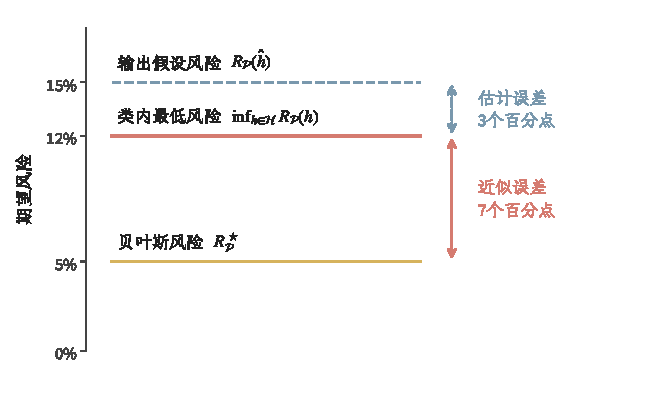
\includegraphics[width=\linewidth,trim=0 8mm 0 0,clip]{figures/02-foundations/02-learning-theory/matplotlib/risk-decomposition.pdf}

  \caption{近似误差与估计误差的期望风险分解。这个教学示例中，当前输入信息决定的贝叶斯风险为
  5\%；阈值假设空间的表达限制把空间内最低期望风险提高到12\%，二者相差7个百分点；学习
  算法依据有限样本得到的分类器的期望风险为15\%，又比空间内最低期望风险高3个百分点。实线与虚线
  分别标出近似误差和估计误差。}
  \label{fig:approximation-estimation-error}
\end{figure}

更丰富的假设空间通常能降低近似误差，因为它拥有更多假设；但学习算法也更容易在有限
样本中找到偶然拟合良好的函数，使估计误差难以控制。这就是所谓的
\term{偏差与复杂度的权衡}（bias--complexity trade-off）：这里的“偏差”指假设空间
的表达限制，“复杂度”指从有限样本中可靠选择假设所付出的统计代价。

以阈值和区间为例，若真实正类由两个分离区间组成，单阈值假设空间即使得到无限数据也会留下
系统性错误，这部分属于近似误差。改用允许许多小区间的假设空间后，训练点可以被细致包围，
近似误差下降；但有限样本没有覆盖到的间隙也可能被误判，估计误差可能增加。扩大假设空间
会改变式~\eqref{eq:approximation-estimation-decomposition}右侧两项，却不必然改善最终期望风险。
结构风险最小化据此要求：选择更丰富的假设空间所带来的拟合改善，应当足以补偿新增的统计不确定性。

\term{经验优化误差}（empirical optimization error）是算法输出的经验风险与假设空间内
最低经验风险之间的差距。例如，训练集中最好的假设只错2封，算法却返回一个错5封的
假设，在这$n$封训练邮件上的平均损失就多出$3/n$。这反映的是训练目标尚未达到最优。它与前面的期望风险分解不是同一个
比较。对输出$\hat h$，经验优化误差定义为
\begin{equation}
  \Delta_{\mathrm{opt}}(S)
  =\hat R_S(\hat h)-\inf_{h\in\mathcal H}\hat R_S(h)
  \geq0,
  \label{eq:empirical-optimization-error}
\end{equation}
这个量比较的是经验目标，不能把式
~\eqref{eq:approximation-estimation-decomposition}任意改写成三个非负期望风险差。后续分析
通常先用泛化界把经验量与期望量联系起来，再说明$\Delta_{\mathrm{opt}}(S)$怎样进入最终
保证。

\subsection{用验证集选择模型}
\label{sec:validation-model-selection}

比较不同复杂度的候选模型时，训练误差只能说明它们对训练样本拟合得怎样。
如果假设空间逐渐扩大，而且每次都求到空间内的最小经验风险，训练误差不会随复杂度
增加而上升；这仍不能保证新样本上的误差也下降。可以另留一份不参与参数拟合的
\term{验证集}，比较候选模型在这些观测上的误差，再据此选择复杂度或其他超参数。
训练、验证与测试的操作边界见第~\ref{sec:experience-data-boundary}节；第一卷关于
选择偏差的讨论进一步说明，最终证据评价的对象应是包含调参在内的整个选择流程，
见\BookSectionRef{sec:statistics-bias-efficiency}{第一卷“随机变量”章的“估计误差与效率”一节}。

图~\ref{fig:learning-model-selection}用一组教学曲线展示这种选择。训练误差持续下降，
验证误差却在复杂度继续增大后回升，因此选择落在最低验证误差处，而不是训练误差
最低处。这里的U形用于说明可能出现的过拟合；实际验证曲线不一定只有一个谷底。
验证集已经参与模型选择，所以还应保留独立的\term{测试集}：锁定模型和超参数后，
只对最终模型作一次评价。反复查看测试误差并据此改模型，会使测试集也参与选择，
失去这次独立评价的作用。

\begin{figure}[htbp]
 \centering
 % 教学构造，不是实验结果。复杂度 t 从 1 到 9：
% training(t)=.3 exp[-.4(t-1)]+.02；validation(t)=.13+.015(t-5)^2。
% 最低验证误差位于 t=5；仅对选定模型标出独立测试误差 .17。
\begin{tikzpicture}[foundation picture]
 \path[use as bounding box] (0,-9) rectangle (112,61);
 \begin{scope}[xshift=4mm]
 \draw[foundation axis] (10,10)--(99,10);
 \draw[foundation axis] (10,10)--(10,52);
 \node[rotate=90] at (1,32) {经验误差};
 \node at (54,-6) {模型复杂度};
 \foreach \error/\label in {0/0,.2/0.2,.4/0.4}{
  \draw[FigureStroke,line width=.9pt] (9,10+80*\error)--(10,10+80*\error);
  \node[anchor=east] at (8,10+80*\error) {$\label$};
 }
 \draw[FigureBlue,line width=1.1pt] (15,57)--(25,57);
 \fill[FigureBlue] (20,57) circle (.9);
 \node[anchor=west] at (27,57) {训练误差};
 \draw[FigureRed,line width=1.1pt,dashed] (59,57)--(69,57);
 \draw[FigureRed,fill=white,line width=1.1pt] (62.9,55.9) rectangle (65.1,58.1);
 \node[anchor=west] at (71,57) {验证误差};
 \draw[FigureBlue,line width=1.1pt,domain=1:9,samples=80]
  plot ({10+10*(\x-1)},{10+80*(.3*exp(-.4*(\x-1))+.02)});
 \draw[FigureRed,line width=1.1pt,dashed,domain=1:9,samples=80]
  plot ({10+10*(\x-1)},{10+80*(.13+.015*(\x-5)^2)});
 \foreach \t in {1,...,9}{
  \pgfmathsetmacro{\tx}{10+10*(\t-1)}
  \pgfmathsetmacro{\trainy}{10+80*(.3*exp(-.4*(\t-1))+.02)}
  \pgfmathsetmacro{\valy}{10+80*(.13+.015*(\t-5)^2)}
  \fill[FigureBlue] (\tx,\trainy) circle (.8);
  \draw[FigureRed,fill=white,line width=1pt] (\tx-.85,\valy-.85) rectangle (\tx+.85,\valy+.85);
 }
 \draw[FigureMuted,line width=.9pt,dotted] (50,10)--(50,20.4);
 \draw[FigureRed,line width=1.1pt] (50,20.4) circle (2.2);
 \node[below] at (50,9) {$\hat k$};
 % 测试误差只在最终锁定的复杂度处出现；不绘制测试曲线。
 \fill[FigureInk] (50,25.2)--(48.7,22.8)--(51.3,22.8)--cycle;
 \node[anchor=center] (testerror) at (77,46) {测试误差};
 \draw[foundation flow,FigureMuted,line width=.9pt] (51.7,24.5)--(testerror.south);
 \end{scope}
\end{tikzpicture}%

 \caption{用验证误差选择模型，再独立测试。实线圆点表示训练误差，虚线方块表示验证误差；
 圆环标出的最低验证误差决定所选复杂度$\hat k$。三角形仅表示选定模型的一次测试误差，
 不参与选择，也不连成测试曲线。曲线和测试点均为人为构造的教学示意，不是实验结果。}
 \label{fig:learning-model-selection}
\end{figure}

\subsection{结构风险最小化}

假设现在有一列逐渐丰富的假设空间
$\mathcal H_1\subseteq\mathcal H_2\subseteq\cdots$。在邮件例子中，
$\mathcal H_k$可以允许至多$k$个区间的并作为正类区域；这样每个假设空间都包含前一个空间中的假设。
如果只按经验风险选择假设空间，空间越丰富，空间内最小经验风险只会下降而不会上升，因而选择
会偏向最丰富的假设空间；如果只为压低估计误差而选择最简单的假设空间，又可能造成很大的近似误差，
也就是偏差。因此，选择假设空间时需要在近似误差（偏差）与估计误差之间进行权衡。

\term{结构风险最小化}（structural risk minimization, SRM）是一种在近似误差与估计误差
之间选择假设空间的方法。这两个期望风险差都依赖未知分布，算法无法直接计算，因此实际采用
带惩罚的经验风险作为选择标准。固定总失败概率$\delta$，给第$k$个假设空间预先分配失败概率
$\delta_k>0$，使$\sum_{k\geq1}\delta_k\leq\delta$。记
$\operatorname{pen}(k,n,\delta_k)$为第$k$个假设空间的复杂度惩罚，结构风险最小化选择
\begin{equation}
  (\hat k,\hat h)
  \in\argmin_{k\geq1,\,h\in\mathcal H_k}
  \left\{\hat R_S(h)+\operatorname{pen}(k,n,\delta_k)\right\}.
  \label{eq:structural-risk-minimization}
\end{equation}
经验风险$\hat R_S(h)$衡量假设在训练样本上的错误，惩罚项则控制从经验风险推断期望风险
时的不确定性。它通常随假设空间复杂度增大而增大，可视为对估计误差的高概率控制量，而不是
估计误差本身。惩罚过小，经验风险较低但只是在样本上偶然拟合良好的复杂假设仍可能胜出；
惩罚过大，选择又会偏向表达能力不足的简单假设空间，造成较大的近似误差（偏差）。若式中的
最小值不能取得，可以像ERM一样使用带惩罚经验目标的近似最小解。

失败概率的分配用于保证所有假设空间可以同时比较。若只让每个假设空间分别以$1-\delta$的概率
估计准确，算法在看过同一份数据后再从许多假设空间中选择，整体失败概率可能超过$\delta$。
将第$k$个假设空间的失败概率限制为$\delta_k$，并使其总和不超过$\delta$，那么至少一个假设空间估计失准的概率就不超过$\sum_k\delta_k\leq\delta$。
于是，以至少$1-\delta$的概率，所有假设空间的经验风险与期望风险都满足各自的偏差要求。

\begin{theorem}[结构风险最小化的期望风险保证]
\label{thm:srm-oracle-bound}
设$\mathcal H_1\subseteq\mathcal H_2\subseteq\cdots$是预先给定的非空假设空间，损失为零一损失，训练样本$S\sim\mathcal P^n$。固定$\delta\in(0,1)$，选择与样本无关的$\delta_k>0$，满足$\sum_{k\geq1}\delta_k\leq\delta$。假设非负惩罚$p_k=\operatorname{pen}(k,n,\delta_k)$使每个假设空间都满足
\begin{equation}
 \mathbb P_{S\sim\mathcal P^n}\left(
 \sup_{h\in\mathcal H_k}
 |R_{\mathcal P}(h)-\hat R_S(h)|>p_k
 \right)\leq\delta_k.
 \label{eq:srm-classwise-confidence}
\end{equation}
这里假定相关事件可测，且惩罚在观察样本前已经确定。

若学习算法输出$\hat h\in\mathcal H_{\hat k}$，并将带惩罚的经验目标求解到给定容差$\rho\geq0$，即
\begin{equation}
 \hat R_S(\hat h)+p_{\hat k}
 \leq\inf_{k\geq1,\,h\in\mathcal H_k}
       \{\hat R_S(h)+p_k\}+\rho,
 \label{eq:srm-approximate-minimizer}
\end{equation}
则以至少$1-\delta$的概率，
\begin{equation}
 R_{\mathcal P}(\hat h)
 \leq\inf_{k\geq1}\left\{
       \inf_{h\in\mathcal H_k}R_{\mathcal P}(h)+2p_k
       \right\}+\rho.
 \label{eq:srm-oracle}
\end{equation}
精确求解式~\eqref{eq:structural-risk-minimization}时，取$\rho=0$。若式~\eqref{eq:srm-classwise-confidence}对所有允许分布使用相同的惩罚都成立，则结论也对这些分布统一成立。
\end{theorem}

\begin{proof}
证明要完成两步：把每个空间的偏差界合成一个同时成立的事件，再在这个事件上，
用带惩罚目标的近似最优性比较算法输出与任意候选。

令$E_k$表示第$k$个假设空间中所有假设都满足$|R_{\mathcal P}(h)-\hat R_S(h)|\leq p_k$的事件，并令$E=\bigcap_{k\geq1}E_k$。至少一个假设空间估计失准的概率不超过各假设空间失准概率之和，因此
\[
 \mathbb P(E^{\mathrm c})
 =\mathbb P\left(\bigcup_{k\geq1}E_k^{\mathrm c}\right)
 \leq\sum_{k\geq1}\mathbb P(E_k^{\mathrm c})
 \leq\sum_{k\geq1}\delta_k\leq\delta.
\]
这个并集界不要求各事件独立；它们可以由同一份训练样本决定。因而$\mathbb P(E)\geq1-\delta$。

现在固定一份属于$E$的样本。由于$E$同时控制所有假设空间，它也控制由数据选出的$\mathcal H_{\hat k}$及其中的输出$\hat h$。于是
\[
 R_{\mathcal P}(\hat h)\leq\hat R_S(\hat h)+p_{\hat k}.
\]
对任意$k$及任意$h\in\mathcal H_k$，近似最优性又给出
\[
 \hat R_S(\hat h)+p_{\hat k}
 \leq\hat R_S(h)+p_k+\rho.
\]
同一个事件$E$还保证$\hat R_S(h)\leq R_{\mathcal P}(h)+p_k$。合并这三次比较，得到
\[
 R_{\mathcal P}(\hat h)
 \leq R_{\mathcal P}(h)+2p_k+\rho.
\]
这里的两个$p_k$都针对用来作参照的$h\in\mathcal H_k$。第一个来自比较带惩罚目标时
给$h$加上的惩罚；第二个来自用$R_{\mathcal P}(h)$替换$\hat R_S(h)$时允许的偏差。
算法输出所在空间的$p_{\hat k}$，已经随其带惩罚目标一起被上面的近似最优性控制。
因此，右侧保留的是参照空间的两项统计代价，而不是把实际估计误差精确拆成这两项。

上式对每个比较假设$h\in\mathcal H_k$以及每个$k$都成立，因此先对$h$、再对$k$取下确界，就得到式~\eqref{eq:srm-oracle}。这一步不要求空间内最优假设或最优假设空间实际存在。整个推导在$E$上成立，而该事件的概率至少为$1-\delta$，故结论成立。
\end{proof}

定理右侧允许用每个假设空间的最好期望风险加上统计代价作比较，尽管算法本身不知道这些期望风险。这样的比较常称为\term{预言机不等式}（oracle inequality）：算法依据可计算的经验目标选择假设空间和假设，却能与假想中知道各空间最低期望风险的选择作比较。这里的“预言机”只是比较基准，并不是训练过程能够调用的额外信息。

例如，可以取$\delta_k=\delta/[k(k+1)]$，因为$1/[k(k+1)]=1/k-1/(k+1)$，求和恰为1。若各$\mathcal H_k$有限，第~\ref{sec:binary-uniform-convergence}节的有限假设空间一致收敛界允许取
\[
 p_k=\sqrt{\frac{\log(2|\mathcal H_k|/\delta_k)}{2n}}
 =\sqrt{\frac{\log(2|\mathcal H_k|)+\log(k(k+1)/\delta)}{2n}}.
\]
其中$|\mathcal H_k|$反映在空间内选择假设的代价，$\delta_k$的分配还计入同时比较多个假设空间的代价。对于无限假设空间，需要用后面的容量工具另行建立式~\eqref{eq:srm-classwise-confidence}，不能把无限的假设数直接代入这个有限空间公式。

式~\eqref{eq:srm-oracle}减去贝叶斯风险后，右侧每个比较项都成为相应假设空间的近似误差加上
$2p_k$，再加求解容差$\rho$。其中近似误差就是该假设空间的偏差，$2p_k$则是控制假设空间选择所产生
估计误差的统计项，并不是估计误差的精确值。假设空间太小可能留下较大偏差，过于复杂则通常需要
较大的统计项。定理保证算法输出假设的期望风险受这些比较项中最好者控制，并不保证总能达到零期望风险，
也没有保证带惩罚目标能够被高效求解。

\section{研究内容}
\label{sec:learning-theory-research-content}

\subsection{发展历史}

机器学习理论并不是从一个统一定义出发建立的。它继承了统计推断关于有限样本、估计误差
和重复抽样的研究，也接住了模式识别与人工智能提出的另一类问题：算法除了估计预先指定的低维参数，还要从许多可能的规则中选择一个用于未见样本。对每条固定规则分别证明
经验频率收敛还不够，因为算法会看过同一批数据以后再选择规则；真正需要控制的是这种
数据依赖选择会增加多少偏差。

这个区别把研究对象从单个估计量推进到整个候选函数类。Vapnik与Chervonenkis把函数类在
有限输入上能够实现多少种划分，与经验频率能否一致逼近总体概率联系起来，使“候选空间不能
过于丰富”成为可计算和可证明的条件\scite{vapnik1971}。这条路线把概率论中的大数规律、
经验过程的统一控制与组合数学中的划分计数连接起来，后来形成了以VC维和一致收敛分析分类
学习的基本框架。它回答的不只是某个分类器估计得准不准，而是同一份样本能否同时支持对
所有候选分类器的比较。

Valiant在1984年提出PAC学习，把“能够从例子中学习”写成算法、样本量、误差容限和失败
概率之间的量词关系，并同时关注样本量与运行时间是否为多项式\scite{valiant1984}。
从此，可学习性不再只表示某个估计量在极限下收敛，而要求一种算法对允许问题族给出统一
的有限样本保证。围绕这一标准，研究者建立了有限假设空间、VC维、经验风险最小化和样本
复杂度之间的联系，也逐步区分统计上存在学习器、存在可计算学习器以及存在高效学习器。

PAC框架带来的关键变化，是把“学会”从经验现象改写成可以比较的成功标准。精度参数说明
风险或超额风险允许偏离目标多少，置信参数说明抽到不利样本的概率可以多大，样本复杂度则追问达到这两个
要求需要多少观测。算法、分布族和样本量之间的量词顺序决定结论强弱：对每个分布分别存在
一个算法，与存在一个算法统一处理全部允许分布，并不是同一项保证。本章前面对PAC定义的
展开，正是对这套历史语言的继承。

统一的成功标准也暴露出统计与计算之间的分工。某个假设空间可能只需少量样本就能区分低
风险规则，却没有已知的高效程序找到它们；反过来，一个优化程序可以迅速降低训练损失，
却未必获得较低的期望风险。计算学习理论因而同时研究表示、查询、归约和运行时间，把
“信息足够”与“程序能够利用这些信息”分成两个问题。这种区分后来不断重现于非凸优化、
大规模训练和组合输出空间。

容量研究随后从最坏情形的组合计数扩展到更贴近数据和函数值的刻画。Rademacher复杂度
利用随机符号测量函数类在当前样本上的拟合能力，可以处理实值预测与替代损失
\scite{bartlettmendelson2002}；伪维、胖打散维和覆盖数把类似思想推广到一般函数类。
样本压缩则从另一方向追问，一份训练样本能否由少量代表观测和有限旁信息重构出可推广的
假设。多分类研究进一步发现，控制一致收敛的维度、刻画可学习性的维度以及不同ERM规则的
样本复杂度不必完全一致，标签结构和输出范围也会改变结论。

这一扩展回应了早期容量刻画的两个限制。VC维只记录二元划分在最坏输入集合上的丰富程度，
却不直接利用当前样本的几何、预测分值或损失变化；实值函数和间隔方法则需要保留这些信息。
数据相关复杂度由此把“函数类最多能有多复杂”改成“它在当前样本附近实际表现出多大波动”，
覆盖数、随机复杂度和间隔界也开始承担不同层次的控制职责。它们没有取消最坏情形理论，而是
在统一保证与贴近具体数据的保证之间增加了选择。

结构风险最小化把容量控制接入模型选择：经验拟合更好的空间可能同时带来更大的选择误差，
因此需要用随空间复杂度增长的惩罚比较不同候选。这个思路使近似误差、估计误差与优化误差
逐步分开。模型太简单时，即使获得无限数据也可能无法逼近目标；模型过于丰富时，有限样本
难以区分偶然拟合与稳定规律；优化没有完成时，算法还可能没有到达统计分析假定的候选。
三类误差后来成为连接学习理论、模型设计和训练算法的共同语言。

样本压缩和多分类结果又说明，函数类的可学习性不一定只能由一种维度解释。一个算法若能把
训练集概括成少量代表样本，就可能直接把可传递的信息量转成泛化保证；标签空间具有结构时，
不同维度则分别控制一致收敛、特定ERM规则和一般学习器。研究由此开始区分“某种证明工具
足以给出保证”与“这个工具完整刻画了可学习性”，避免把二分类中的等价关系未经检查地推广
到所有输出空间。

\Needspace{18\baselineskip}
只分析整个假设空间，仍难解释具体算法为何从庞大空间中选出可推广的结果。算法稳定性把
对象转向删除或替换一条样本以后输出怎样变化，Bousquet与Elisseeff系统建立了稳定性与
泛化的联系；后续工作进一步用稳定性刻画一般学习问题，并分析随机梯度下降中的扰动传播
\scite{bousquetelisseeff2002,shalevshwartz2010learnability,hardt2016sgd}。信息论路线
则用算法输出携带了多少训练数据的信息控制期望泛化差，使互信息、条件互信息和换测度工具
进入学习理论\scite{xu2017information}。这些工作把“空间是否太大”扩展成“算法实际选择
了什么、对数据有多敏感”。

稳定性分析保留了训练过程的差异。同一个函数空间可以由正则化经验风险最小化、随机梯度
下降或另一套选解规则处理，它们在替换一条样本后可能产生完全不同的输出变化。稳定性小，表示单条样本的替换对结果影响有限；这回答的是泛化差怎样控制，还没有
回答训练目标是否求得足够好。

信息论分析则把“记住了多少样本细节”变成分布之间的可计算差异。普通互信息适合控制算法
输出与整份样本的平均依赖，条件互信息可以在预先抽取的双样本中比较算法透露了哪些选择，
压缩长度和有限输出范围还可转成信息量上界。这些工具通常先给出期望泛化差，若要得到PAC
意义下的高概率保证，仍需集中分析、尾界或由期望到概率的额外步骤。

两种方法都还需要评价训练是否有效：一个始终输出同一决策的算法，可能既稳定，
又与训练数据几乎无关，却把任务做得很差。因此，泛化差的控制必须配合经验拟合和
比较基准，才能说明算法学到了有用规律。

算法依赖视角还改变了理论与训练记录的关系。函数类容量通常在训练前就能定义，稳定性和
信息量却取决于算法如何随机化、运行多少步以及最终输出什么。理论开始需要保存初始化、
样本顺序、迭代轨迹和停止规则，才能判断同一模型空间中的两个训练过程为何得到不同保证。
这为后来按优化轨迹、参数分布和表示变化分析深度网络准备了方法，也使“模型复杂度”逐渐
从一个静态数值变成与训练过程共同确定的对象。

\Needspace{20\baselineskip}
深度学习把这种转向推到更突出的位置。现代网络能够拟合随机标签，说明参数数量和表达能力
不能单独解释泛化\scite{zhang2021rethinking}。研究者因而从权重范数与分类间隔、初始化
附近的神经切线核、梯度下降的隐式偏差、宽网络的平均场极限以及完整参数分布的
PAC--Bayes分析等角度研究选解\scite{jacot2018ntk,soudry2018implicit,maurer2004pacbayes}。
这些路线都把学习理论与优化动力学连接起来：模型能否表示目标、训练能否降低经验风险、
算法偏向哪个解以及该解能否泛化，是彼此相关但不能互相替代的问题。

\Needspace{16\baselineskip}
过参数化网络使传统的“参数少于样本才可能泛化”直觉失去普遍性。网络可以达到近乎零训练
误差，测试风险却可能在模型规模继续增加时再次下降；线性插值模型中的良性过拟合研究表明，
这种现象在协方差谱、噪声和最小范数选解满足特定条件时也能出现
\scite{belkin2019double,bartlett2020benign}。这并不说明复杂度不再重要，而是说明原始
参数个数没有记录数据几何、优化偏好，以及所选解中实际影响预测的独立变化方向有多少。理论任务因而从排除插值，转向
说明何种插值解能够控制噪声并保留可推广结构。

不同路线观察的是不同训练区域。神经切线核研究参数停留在初始化邻域时，网络怎样近似一个
由初始梯度决定的核方法；隐式偏差研究显式正则化缺席时，优化轨迹为何仍偏向某类解；
平均场分析关注宽度增加时参数分布的演化；PAC--Bayes则比较数据相关的参数分布与事先选定
的参照分布。它们可以在特定模型上相互印证，却不能把一个区域内的近似结论直接推广到发生
显著特征学习的训练过程。

随着预训练模型扩大数据、参数和计算规模，学习理论又需要追踪更完整的学习流程。预训练数据决定
初始表示，优化过程决定哪些能力被形成或保留，下游样本只在这个表示上完成有限调整，推理
阶段还可能通过上下文示例和额外计算改变输出。一个下游风险数值同时混入了预训练覆盖、
表示充分性、适应算法和评价协议。研究因此不能只计算微调阶段的参数量，而要追踪知识在
预训练、迁移和推理各阶段由什么信息支持。

\Needspace{8\baselineskip}
同分布假设之外，领域自适应与领域泛化把训练数据能否支持目标环境的问题单独提出。
相关理论用分布差异、覆盖、共享标签机制和共同错误等条件连接源域与目标域，同时证明缺少
这些联系时，即使假设空间很小，也可能无法识别目标标签
\scite{bendavid2010adaptation,bendavid2010impossibility}。这一发展使机器学习理论与因果
推断中的可识别性、时间序列中的依赖、在线学习中的动态比较及鲁棒优化中的不确定集合发生
更直接的交叉。

分布差异项只能描述观测到的输入或预测关系相差多少，不能凭空确定目标域的正确标签。
如果源域与目标域在输入支持上缺少覆盖，或者同一输入在两个环境中对应不同目标，任何只看
无标签目标输入的算法都可能面对彼此不可区分、却要求相反预测的世界。迁移理论因此要先写
清共享机制和可识别性，再讨论有限样本复杂度；把差异估计得更精确不能补回根本缺失的信息。

从一个源域到一个目标域的设定，后来又扩展为多环境训练、持续变化和测试时适应。多个训练
环境可以帮助区分偶然相关与跨环境稳定关系，却只有在环境差异真正提供了辨别信息时才有用；
在线更新能够利用近期数据，也会使算法输出、样本选择和评价分布共同变化。这里的核心困难
不再只是给一个固定分布上的经验风险加误差项，而是说明环境如何产生、哪些机制保持不变，
以及新数据何时足以识别已经发生的变化。

回看这段历史，机器学习理论的研究对象经历了几次相互叠加的扩大：从固定规则的估计误差，
到函数类的统一控制；从样本复杂度，到计算能否实现；从最坏情形容量，到算法实际选择的解；
从同一分布上的泛化，到变化环境中的可识别性。后来的路线没有简单淘汰前面的工具。相反，
每次扩大都保留了原问题，并要求更明确地说明数据从哪里来、算法看到了什么、比较基准是谁，
以及结论对哪些随机性成立。后面的“当前前沿”小节，正是在这些历史分层上继续展开。

\subsection{当前前沿}

机器学习理论研究有限经验在什么信息、统计和计算条件下能够支持可推广的学习。图~
\ref{fig:learning-theory-research-problems-map}由共同判断向外展开研究内容：内环给出
问题与信息、泛化机制、实现与扩展三类条件，中环组织八个相互制约的问题，外环列出其中
部分问题下的代表课题。下面不再逐项复述这些基础问题，只讨论仍在快速发展的主要方向及其
尚未解决的挑战。

\begin{figure*}[htbp]
  \centering
  % 机器学习理论研究地图：中心问题、三类条件、八个研究问题与十五项具体课题。
\begingroup
\newcommand{\theorysector}[5]{%
  \path[fill=#5,draw=black,line width=.75pt]
    (#1:#4) arc[start angle=#1,end angle=#2,radius=#4]
    -- (#2:#3) arc[start angle=#2,end angle=#1,radius=#3] -- cycle;}
\newcommand{\theorylabel}[5][]{%
  \node[font=\figurefont\mdseries#1,text=FigureInk,align=center,
    rotate=#5,transform shape] at (#2:#3) {#4};}

\begin{tikzpicture}[figure picture,foundation picture]
  \path[use as bounding box] (-82,-82) rectangle (82,82);

  % 第一层：学习问题与信息、泛化机制、实现与扩展。
  \theorysector{90}{-45}{16}{34}{FigureBlue!78!white}
  \theorysector{-45}{-180}{16}{34}{FigureYellow!82!white}
  \theorysector{-180}{-270}{16}{34}{FigureRed!78!white}

  % 第二层：八个相互制约的研究问题。
  \theorysector{90}{45}{34}{55}{FigureBlue!58!white}
  \theorysector{45}{0}{34}{55}{FigureBlue!58!white}
  \theorysector{0}{-45}{34}{55}{FigureBlue!58!white}
  \theorysector{-45}{-90}{34}{55}{FigureYellow!62!white}
  \theorysector{-90}{-135}{34}{55}{FigureYellow!62!white}
  \theorysector{-135}{-180}{34}{55}{FigureYellow!62!white}
  \theorysector{-180}{-225}{34}{55}{FigureRed!58!white}
  \theorysector{-225}{-270}{34}{55}{FigureRed!58!white}

  % 第三层：每个类别内部顺时针展开，末项在中层收束。
  \foreach \a/\b in {90/75,75/60,60/45,45/30,30/15,15/0}
    {\theorysector{\a}{\b}{55}{80}{FigureBlue!34!white}}
  \foreach \a/\b in {-45/-60,-60/-75,-75/-90,-90/-105,-105/-120,-120/-135}
    {\theorysector{\a}{\b}{55}{80}{FigureYellow!38!white}}
  \foreach \a/\b in {-180/-195,-195/-210,-210/-225}
    {\theorysector{\a}{\b}{55}{80}{FigureRed!34!white}}

  % 中心问题。
  \fill[white] (0,0) circle[radius=16];
  \draw[draw=black,line width=1pt] (0,0) circle[radius=16];
  \node[font=\figurefont\mdseries\fontsize{8.8}{10.5}\selectfont,
    text=FigureInk,align=center,text width=28mm] at (0,0)
    {\bfseries 机器学习理论\\[1mm]
     有限经验如何支持\\可计算、可推广的\\学习？};

  % 第一层标签。
  \theorylabel[\fontsize{8.2}{9.8}\selectfont]{22.5}{25}{问题与信息}{-67.5}
  \theorylabel[\fontsize{8.2}{9.8}\selectfont]{-112.5}{25}{泛化机制}{-22.5}
  \theorylabel[\fontsize{8.2}{9.8}\selectfont]{-225}{25}{实现与扩展}{45}

  % 第二层标签。
  \theorylabel[\fontsize{7.3}{8.8}\selectfont]{67.5}{44.5}{目标\\可识别性}{-22.5}
  \theorylabel[\fontsize{7.3}{8.8}\selectfont]{22.5}{44.5}{输出、标签\\与损失结构}{-67.5}
  \theorylabel[\fontsize{7.3}{8.8}\selectfont]{-22.5}{44.5}{分布变化\\与适应}{67.5}
  \theorylabel[\fontsize{7.3}{8.8}\selectfont]{-67.5}{44.5}{样本与\\复杂度}{22.5}
  \theorylabel[\fontsize{7.3}{8.8}\selectfont]{-112.5}{44.5}{表示与\\预训练}{-22.5}
  \theorylabel[\fontsize{7.3}{8.8}\selectfont]{-157.5}{44.5}{算法\\选解}{-67.5}
  \theorylabel[\fontsize{7.3}{8.8}\selectfont]{-202.5}{44.5}{规模与\\能力变化}{67.5}
  \theorylabel[\fontsize{7.3}{8.8}\selectfont]{-247.5}{44.5}{计算、资源\\与验证}{22.5}

  % 外层标签：问题与信息。
  \theorylabel[\fontsize{6.5}{7.7}\selectfont]{82.5}{67.5}{观测机制}{-7.5}
  \theorylabel[\fontsize{6.5}{7.7}\selectfont]{67.5}{67.5}{归纳偏置}{-22.5}
  \theorylabel[\fontsize{6.5}{7.7}\selectfont]{52.5}{67.5}{反馈与\\可识别}{-37.5}
  \theorylabel[\fontsize{6.5}{7.7}\selectfont]{37.5}{67.5}{标签结构}{-52.5}
  \theorylabel[\fontsize{6.5}{7.7}\selectfont]{22.5}{67.5}{恰当与\\非恰当}{-67.5}
  \theorylabel[\fontsize{6.5}{7.7}\selectfont]{7.5}{67.5}{损失与解码}{-82.5}

  % 外层标签：泛化机制。
  \theorylabel[\fontsize{6.5}{7.7}\selectfont]{-52.5}{67.5}{随机复杂度}{37.5}
  \theorylabel[\fontsize{6.5}{7.7}\selectfont]{-67.5}{67.5}{压缩与信息}{22.5}
  \theorylabel[\fontsize{6.5}{7.7}\selectfont]{-82.5}{67.5}{有效样本\\单位}{7.5}
  \theorylabel[\fontsize{6.5}{7.7}\selectfont]{-97.5}{67.5}{预训练表示}{-7.5}
  \theorylabel[\fontsize{6.5}{7.7}\selectfont]{-112.5}{67.5}{上下文学习}{-22.5}
  \theorylabel[\fontsize{6.5}{7.7}\selectfont]{-127.5}{67.5}{长度与序列}{-37.5}

  % 外层标签：实现与扩展。
  \theorylabel[\fontsize{6.5}{7.7}\selectfont]{-187.5}{67.5}{缩放定律}{82.5}
  \theorylabel[\fontsize{6.5}{7.7}\selectfont]{-202.5}{67.5}{阈值与涌现}{67.5}
  \theorylabel[\fontsize{6.5}{7.7}\selectfont]{-217.5}{67.5}{顿悟与\\推理计算}{52.5}

  % 统一外轮廓与层级边界。
  \draw[draw=black,line width=.8pt]
    (90:80) arc[start angle=90,end angle=0,radius=80];
  \draw[draw=black,line width=.8pt]
    (-45:80) arc[start angle=-45,end angle=-135,radius=80];
  \draw[draw=black,line width=.8pt]
    (-180:80) arc[start angle=-180,end angle=-225,radius=80];
  \foreach \a in {90,0,-45,-135,-180,-225}
    {\draw[draw=black,line width=.8pt] (\a:55) -- (\a:80);}
  \draw[draw=black,line width=.6pt] (0,0) circle[radius=34];
  \draw[draw=black,line width=.6pt] (0,0) circle[radius=55];
\end{tikzpicture}%
\endgroup

  \begingroup
    \let\RaggedRight\Centering
    \caption{机器学习理论分层研究地图。}
    \label{fig:learning-theory-research-problems-map}
  \endgroup
\end{figure*}

\Needspace{20\baselineskip}
\paragraph{数据与算法相关的泛化解释}

现代模型的最坏情形容量通常远大于样本量，统一上界即使正确，也未必解释实际训练得到的
模型为何能够推广。当前研究转向间隔、范数、压缩长度、稳定性、信息依赖、参数后验和完整
训练轨迹，希望刻画算法真正到达的解，而不是整个候选空间。核心挑战是这些量往往由同一
训练数据选择，还会随参数化和优化器改变；训练后数值较小，只有在选择过程与概率依赖得到
控制时，才构成有效的泛化证据。

大语言模型又使样本单位和数据依赖变得含混。文档、序列、词元和上下文窗口并非独立观测，
把每个词元都计作一个样本可能夸大有效信息量。近期工作尝试利用参数后验或更细的数据分解
得到数值上能提供实际判断依据的语言模型泛化界\scite{lotfi2024llm,lotfi2024tokens}，但结论仍取决于条件
独立性、先验的确定方式和数据选择过程。怎样同时得到数值有解释力、条件可验证且能预测
更换优化器或停止时间后风险怎样变化的界，仍是这一方向的主要困难。

另一项挑战是从相关指标走向机制。平坦性、频谱或某种稳定性可能与测试表现相关，却未必
解释改变初始化、样本顺序或训练时长后为何发生变化。前沿研究正在把最终参数统计与训练
动力学连接起来，要求理论不仅拟合已经观察到的结果，还能预测受控干预后的选解和风险。

\Needspace{10\baselineskip}
\paragraph{预训练、上下文学习与表示迁移}

预训练把大量外部经验带入下游任务，使样本复杂度不再只由微调阶段的可训练参数决定。冻结
表示可以减少优化自由度，却可能丢失目标信息；开放更多参数提高适应能力，也会增加数据依赖
和遗忘风险。当前研究需要分别检查：只调整较少参数，是否也减少了获得目标效果所需的带标签样本。
这分别对应参数效率与统计效率；还要量化预训练数据、表示选择和下游监督
分别提供了多少任务信息。

上下文学习进一步把“训练”和“使用”的边界变得模糊。模型参数保持不变，却能根据提示中的
示例改变预测；理论既可以把这种行为解释为隐式贝叶斯推断，也可以把Transformer看作执行
某类学习算法\scite{xie2022bayesianicl,li2023icl}。这些解释需要明确预训练分布、上下文
生成方式和任务族，不能从受控模型中的机制直接推出任意基础模型都采用同一过程。

上下文中的示例通常有顺序和依赖，新增一个示例还可能同时改变注意力分配与输出长度。近期
稳定性与非独立同分布泛化分析尝试控制示例替换和依赖结构，长度泛化研究则追问训练长度之外
的计算能否保持规则\scite{wang2026iclstability,huang2025length}。这些问题把表示能力、
算法模拟和序列外推放在同一分析中。主要挑战是把受控模型中的解释推进到真实预训练系统：
预训练语料通常不透明，上下文示例也会改变注意力和输出长度，观察到的适应行为未必由单一
机制产生。

\Needspace{16\baselineskip}
\paragraph{统计、计算与可验证性的统一}

样本最优并不等于计算可行，训练可行也不等于通信、存储和预测成本适合实际使用。理论分析
常调用优化预言机、独立采样器或无限精度运算；把这些对象换成有限迭代和有限资源实现时，
需要重新计入优化误差、随机误差与停止条件。当前前沿正在联合分析样本、时间、内存和通信
预算，避免把统计存在性直接解释为可执行算法。

另一项挑战是缩小理论条件与可检查证据之间的距离。范数、覆盖常数、稳定性或分布差异若
只能在未知总体上定义，就难以判断定理是否适用于当前系统。研究需要把不可观测假设与可由
训练日志、独立数据、重复运行或干预检验的条件分开，并计算验证本身所需的样本和资源。

\Needspace{10\baselineskip}
\paragraph{规模规律、能力变化与测试时计算}

大模型实验常同时增加参数量、训练数据和计算预算。\term{缩放定律}（scaling law）记录这些资源与测试损失之间的
经验关系，并用于预算分配\scite{kaplan2020scaling,hoffmann2022chinchilla}。这类关系
首先是对已观察区间的描述，不是无条件外推定理。数据重复、优化未收敛、模型形状和评价集
污染都可能改变曲线，参数、词元和计算量同时变化时，也难以仅凭拟合曲线识别主导机制。

相似的幂律曲线可能来自近似误差、估计误差、优化进度或特征学习。要区分这些解释，需要预测改变数据协方差的特征值分布、训练时长或模型形状后会怎样。所谓能力突现也可能来自评价时设置的达标阈值：连续改善的分数一旦越过阈值，看起来就像能力突然出现。\term{顿悟}（grokking）则指模型已拟合训练数据后，仍继续训练很久才出现明显泛化改善的现象；解释它还需考察特征形成、隐式偏差和测量尺度\scite{bordelon2025featurelaws,schaeffer2023emergence,power2022grokking}。许多机制都可能重现一条曲线，能对新实验给出不同的预测，才有助于判断哪种解释更合适。

推理阶段增加采样、搜索或验证计算，又把规模变量从训练扩展到使用。增加测试时计算可能在
特定推理任务和策略下改善结果\scite{snell2025testtime}，但其收益同时依赖候选生成、
选择器质量和计算预算。理论需要把“模型参数更大”和“同一模型搜索更久”分开，研究计算怎样
改变错误相关性、选择偏差和最终风险。当前挑战是建立能够跨资源区间外推、又能区分训练规模
与测试时搜索机制的理论。

\Needspace{10\baselineskip}
\paragraph{变化环境中的持续学习保证}

预训练使“未见环境”更难界定。模型可能在大规模预训练中接触过相同来源、相近样本或目标
任务线索，只看微调数据无法判断迁移来自共享结构还是既有覆盖。领域泛化评价若忽略预训练
暴露，可能把已有经验误写成对未见分布的外推\scite{mayilvahanan2025domaingeneralization}。
当前理论与评价协议都需要记录预训练来源、模型选择所见环境和最终测试环境，并说明哪些
跨域关系足以识别目标风险。

持续变化又使一次源域到目标域的比较不够。测试时适应会根据近期输入更新模型，更新后的
输出反过来影响下一批可见数据；无标签代理目标可能在变化后失去任务含义，攻击者也可能
操纵更新流。恢复复杂度尝试量化变化后重新达到给定性能需要多少代价
\scite{zhou2026ttalearnability}；变化下的共形方法则开始研究协变量和后验同时漂移时的
覆盖\scite{wang2025conformalshift}。两类结果都必须写明变化范围、允许反馈和加权误差，
不能由过去的交换性结论直接推出。

这一方向的共同挑战是处理时间依赖和自适应交互。理论不仅要界定变化后还能保证什么，还要
联合控制检测延迟、更新稳定性、历史任务退化和恢复时间，并规定何时停止适应或回退。这些问题正在把经典可学习性推进到更贴近实际算法、资源和数据过程的保证，同时要求
假设能够被检查，结论的失效条件能够被明确记录。

\section{本章小结}
\label{sec:statistical-framework-summary}

要判断有限样本能否支持对未来表现的推断，必须先明确学习问题的观测单位、比较空间、
算法输出、损失、允许分布族和随机来源。特化到二分类后，学习算法能够直接比较的是
样本上的经验风险，需要保证的却是未来数据上的期望风险。PAC模型把这项要求写成两个
明确的目标：输出假设的期望风险或超额期望风险不超过误差容限，训练失败的概率不超过
失败概率容限$\delta$，也就是成功概率至少达到置信水平$1-\delta$。可实现设定以零期望
风险为基准；不可知设定允许标签噪声与假设空间的表达限制，以空间内期望风险的下确界
为基准。两种保证都要求所给样本量适用于全部允许分布。

经验风险最小化并不自动满足这些要求。没有免费的午餐定理说明，若假设空间允许未见
输入的标签任意变化，有限观测就不足以可靠预测；增加计算资源不能补足缺失的信息。
限制假设空间有助于利用样本，却也可能排除期望风险较低的假设。贝叶斯风险、近似误差
与估计误差的分解，分别说明现有输入信息、假设空间与学习结果对最终期望风险的影响。
其中，估计误差比较两个期望风险，不能与经验风险或泛化差混用。

学习理论的发展从控制候选空间的容量，推进到分析算法稳定性、信息依赖和深度网络选解，
再扩展到训练与评价分布不同的情形。后续各章分别改变标签结构、损失、参数化和数据关系，
共同检查信息可识别性、表示能力、有限样本误差与计算实现。规模规律、持续适应等热点并未
取消这些基本问题，反而要求更准确地说明任务、概率来源和能够验证的条件。

结构风险最小化用经验风险与复杂度惩罚共同选择假设空间。它的保证依赖各空间的
经验风险与期望风险偏差能否被控制；下一章将为二分类问题建立这种控制所需的容量条件。
即使样本量条件已经成立，能否用可停机、运行时间可接受的程序完成学习，仍是另一项要求。

\paragraph{延伸阅读}
Shalev-Shwartz与Ben-David的\textit{Understanding Machine Learning}第2--5章系统展开了
PAC模型、经验风险最小化与没有免费的午餐定理，第7章进一步讨论结构风险最小化和描述长度。
阅读时可以对照本章检查每个结论的比较基准，以及先固定算法、再对分布和样本作保证的
量词顺序；这些约定也决定了后续定理应如何解释\scite{shalevshwartz2014}。

若希望继续区分统计可学习性与程序可计算性，可阅读Delle Rose等关于可计算PAC学习的研究。
其中的有效见证条件说明，统计上知道某种预测不可能出现，与能够写程序找出这种预测，
是两项不同的要求。第~\ref{sec:computable-binary-learning}节将给出相应定义与例子\scite{dellerose2023}。
